\documentclass[aps,showpacs,twocolumn,prd,superscriptaddress,nofootinbib]{revtex4-1}

\usepackage{amsmath}
\usepackage{amsfonts}
\usepackage{amssymb}
\usepackage{latexsym}
\usepackage{graphicx}
\usepackage{bm}
%\usepackage{color}
\usepackage{enumerate}
\usepackage{ulem}
\usepackage{tabularx}
\usepackage{braket}

\usepackage{color}
\usepackage[usenames,dvipsnames,svgnames,table]{xcolor}
%\usepackage[colorlinks=true,
%            linkcolor=green,
%            urlcolor=blue,
%            citecolor=red]{hyperref}
\usepackage[colorlinks=true,
            linkcolor=YellowOrange,
            urlcolor=RoyalBlue,
            citecolor=RedViolet]{hyperref}

\newcommand{\be}{\begin{equation}}
\newcommand{\ee}{\end{equation}}
\newcommand{\bsub}{\begin{subequations}}
\newcommand{\esub}{\end{subequations}}
\newcommand\ud{{\mathrm{d}}}
\newcommand\uD{{\mathrm{D}}}
\newcommand\calO{{\mathcal{O}}}
\newcommand\calM{{\mathcal{M}}}
\newcommand\calF{{\mathcal{F}}}
\newcommand\calT{{\mathcal{T}}}
\newcommand\calD{{\mathcal{D}}}
\newcommand\calA{{\mathcal{A}}}
\newcommand\calL{{\mathcal{L}}}
\newcommand\bfx{\mathbf{x}}
\newcommand{\ov}[1]{\overline{#1}}
\newcommand{\ph}[1]{\phantom{#1}}
\newcommand{\cte}{\mathrm{cte}}
\newcommand{\nn}{\nonumber}
\newcommand{\hatk}{\hat{k}}
\newcommand{\Hz}{\,\mathrm{Hz}}
\newcommand{\sinc}{\,\mathrm{sinc}}
\newcommand{\Msol}{M_{\odot}}
\newcommand{\Mchirp}{M_{c}}
\newcommand\betaL{{\beta_{L}}}
\newcommand\lambdaL{{\lambda_{L}}}
\newcommand\varphiL{{\varphi_{L}}}
\newcommand\psiL{{\psi_{L}}}
\newcommand{\tf}{t_{f}}
\newcommand{\Tf}{T_{f}}
\newcommand{\tfd}{t_{f}^{d}}
\newcommand{\tfSPA}{t_{f}^{\rm SPA}}
\newcommand{\TfSPA}{T_{f}^{\rm SPA}}
\newcommand{\sYlm}{{}_{-2}Y_{\ell m}}
\newcommand{\sYlmstar}{{}_{-2}Y_{\ell m}^{*}}
\newcommand{\sYlminusmstar}{{}_{-2}Y_{\ell, -m}^{*}}

\newcolumntype{C}[1]{>{\centering\arraybackslash}p{#1}}
\newcolumntype{L}[1]{>{\raggedright\arraybackslash}p{#1}}

\newcommand{\SM}[1]{{\color{Blue} [SM: #1]}}
\newcommand{\JGB}[1]{{\color{DarkGreen} [JGB: #1]}}
\newcommand{\TDC}[1]{{\color{red} [TDC: #1]}}

\begin{document}

%\title{Bayesian methods for black hole merger parameter estimation with LISA.}
\title{Exploring Bayesian parameter estimation of binary black holes with LISA}

\author{Sylvain Marsat}
\affiliation{APC, AstroParticule et Cosmologie, Universit\'{e} Paris Diderot, CNRS/IN2P3, CEA/Irfu, Observatoire de Paris, Sorbonne Paris Cit\'{e}, 10, rue Alice Domon et L\'{e}onie Duquet 75205 PARIS Cedex 13, France}
\author{John G. Baker}
\affiliation{Gravitational Astrophysics Laboratory, NASA Goddard Space Flight Center, 8800 Greenbelt Rd., Greenbelt, MD 20771, USA}
\author{Tito Dal Canton}
\thanks{NASA Postdoctoral Program fellow}
\affiliation{Gravitational Astrophysics Laboratory, NASA Goddard Space Flight Center, 8800 Greenbelt Rd., Greenbelt, MD 20771, USA}


\date{\today}

\begin{abstract}

The space-based gravitational wave detector LISA will observe mergers of supermassive black hole binary systems (SMBHs) to cosmological distances, as well as inspiralling stellar-origin (or stellar-mass) binaries (SOBHs) years before they enter the LIGO/Virgo band. Much remains to be explored for the parameter recovery of both class of systems. Previous SMBH analyses relied on inspiral-only signals and/or a simplified Fisher matrix analysis, while SOBHs have not yet been analyzed with Bayesian methods. We accelerate likelihood computations by (i) using a Fourier-domain response of the LISA instrument, (ii) using a reduced-order model for non-spinning waveforms that include a merger-ringdown and higher harmonics, (iii) setting the noise realization to zero and computing overlaps in the amplitude/phase representation. We present the first simulations of Bayesian inference for the parameters of supermassive black hole systems including consistently the merger and ringdown of the signal, as well as higher harmonics. We find that restricting the merger-dominated signal to its dominant harmonic can make the extrinsic likelihood very degenerate. Including higher harmonics proves to be crucial to break degeneracies and considerably improves the localization of the source, with a surviving bimodality in the sky position. We also present the first simulations of Bayesian inference for SOBHs, and show that although unimodal, their posterior distributions can have non-Gaussian features.

\end{abstract}

\pacs{
04.70.Bw, % classical black holes
04.80.Nn, % Gravitational wave detectors and experiments
95.30.Sf, % relativity and gravitation
95.55.Ym, % Gravitational radiation detectors
97.60.Lf  % black holes (astrophysics)
}

\maketitle

%%%%%%%%%%%%%%%%%%%%%%%%%%%%%%%%%%%%
%%%%%%%%%%%%%%%%%%%%%%%%%%%%%%%%%%%%

\section{Introduction}
\label{sec:intro}

%The future gravitational wave detector LISA~\cite{LISA2017}.
%
%, the network of ground-based detectors will have expanded from the current LIGO~\cite{} and Virgo~\cite{} detectors to include KAGRA~\cite{} and Indigo, which will have continued improving their sensitivity. By the time LISA will fly, a third generation of detectors, like Einstein Telescope~\cite{} and Cosmic Explorer~\cite{}, might be operating.
%
%LISA will provide complementary informations. By targeting a much lower frequency band, will be sensitive to different sources. Among the sources, mergers of SMBHs, seen at high SNR and anywhere in the observable universe, and inspirals of LIGO-type sources (SOBHs), opening the possibility of multi-band gravitational wave astronomy.
%
%Much remained to be explored for the data analysis of LISA. Different challenges : high SNR for merger-dominated SMBH signals, SNR-limited regime for very long SOBH signals. The motion of the detector leaves an imprint on the signal, while the response also has frequency-dependency at high frequencies where the long-wavelength approx is not valid anymore. Finally, many other challenges : calibration and understanding noise on the fly, non-stationarity of the noise, dealing with glitches, and most importantly global fit: superposition of long-lived sources in a single datastream.



%%%%%%%%%%%%%%%%%%%%%%%%%%%%%%%%%%%%
%%%%%%%%%%%%%%%%%%%%%%%%%%%%%%%%%%%%

\section{Methodology}
\label{sec:method}

%%%%%%%%%%%%%%%%%%%%%%%%%%%%%%%%%%%%

\subsection{Bayesian setting}
\label{subsec:defbayes}

-- definitions relevant to the Bayesian setting (likelihood, ...)

Introducing the standard matched-filter inner product (also called overlap) as
\be\label{eq:definnerproduct}
	( \tilde{a} | \tilde{b} ) = 4 \mathrm{Re} \int_{0}^{+\infty} df \; \frac{\tilde{a}(f) \tilde{b}^{*}(f)}{S_{n}(f)} \,,
\ee
for stationary Gaussian noise with noise PSD $S_{n}$, the likelihood $\calL = p(d | \bm{\theta})$ for a given gravitational wave channel takes the form
\be\label{eq:deflnL}
	\ln \calL = -\frac{1}{2} \left( h(\bm{\theta}) - d | h(\bm{\theta}) - d \right) \,,
\ee
with the data stream being a superposition of the gravitational wave signal for the true parameters $\bm{\theta}_{0}$ and the noise realization in the experiment, $d = h(\bm{\theta}_{0}) + n$. In general, the templates $h(\theta)$ used for the analysis will only be an approximation of the physical signals entering the data stream $d$; we will ignore entirely this distinction and neglect the systematic errors in the waveform model. The posterior distribution for the physical parameters $\bm{\theta}$ given the observed data $d$ is then
\be\label{eq:defBayes}
	p\left( \bm{\theta} | d \right) = \frac{p(d | \bm{\theta})p(\bm{\theta})}{p(d)}\,,
\ee
with $p(\bm{\theta})$ the priors on the parameters, and $p(d)$ the evidence that we will ignore here as it enters as a multiplicative constant in the posterior.

In our analysis, we will use the so-called zero-noise approximation. This corresponds simply to performing a Bayesian analysis with~\eqref{eq:deflnL} and ~\eqref{eq:defBayes}, but setting the noise realization to zero, $n=0$. It allows us to accelerate the likelihood computation, as will be explained in~\ref{}. For exploratory parameter estimation runs, this approximation allows us to explore the structure of the likelihood with its possible parameter degeneracies (\SM{cite past use of this approx.}), and is a significant improvement over Fisher matrix estimates in that sense. We leave the extension of our analysis to include noise realizations for future work. We will also ignore waveform systematic errors and assume our waveform templates match exactly the real signals.

%%%%%%%%%%%%%%%%%%%%%%%%%%%%%%%%%%%%

\subsection{Frequency domain LISA response}
\label{subsec:response}

We will give in this section a brief summary of the instrument response of LISA, and of our Fourier-domain treatment of the modulations and delays. We refer the reader to App.~\ref{app:response} for comprehensive notations and definitions.

The higher harmonics $h_{\ell, m}$ parametrize the decomposition of the gravitational wave signal $h_{+}$, $h_{\times}$ in spin-weighted spherical harmonics as
\be\label{eq:hpcmodes}
	h_{+} - i h_{\times} = \sum_{\ell \geq 2} \sum_{m = -\ell}^{\ell} {}_{-2}Y_{\ell m} (\iota, \varphi) h_{\ell m} \,,
\ee
where $(\iota, \varphi)$ is the direction of emission in a frame attached to the source by convention, and the ${}_{-2}Y_{\ell m}$ are spin-weighted spherical harmonics~\cite{}.

The LISA response can be built from single-link observables $y_{slr} = (\nu_{r} - \nu_{s})/\nu$ respresenting a frequency shift between the spacecrafts $s$ and $r$ along the link $l$. We use the expression~\cite{}
\be\label{eq:defyslr}
	y_{slr} = \frac{1}{2} \frac{n_{l} \otimes n_{l}}{1 - k\cdot n_{l}} : \left[ H(t - L - k\cdot p_{s}) - H(t - k\cdot p_{r}) \right] \,,
\ee
with $H$ the transverse-traceless matrix representing the gravitational wave, $L$ the delay along one arm\footnote{We use units with $G=c=1$.}, taken to be fixed, $k$ the propagation vector, $n_{l}$ the link unit vectors and $p_{r}$, $p_{s}$ the positions of the spacecrafts.

In the frequency domain, modes will be respresented with their amplitude and phase as\footnote{Note our Fourier convention~\eqref{eq:defFourier}.}
\be\label{eq:hlmampphase}
	\tilde{h}_{\ell m} (f) = A_{\ell m} (f) e^{-i\Psi_{\ell m} (f)}\,.
\ee
We will use the analysis of~\cite{MB18} and write the response in individual observables $y_{slr}$ with a transfer function for each spherical harmonic mode as
\be
	\tilde{y}_{slr} = \sum_{\ell, m}\calT_{slr}^{\ell m}(f) \tilde{h}_{\ell m} \,.
\ee
Applying the perturbative formalism of~\cite{MB18} to leading order, we have simply
\be
	\calT_{slr}^{\ell m}(f) = G_{slr}^{\ell m}(f, t_{f}^{\ell m}) \,,
\ee
where
\begin{align}\label{eq:Gslr}
	G_{slr}^{\ell m}(f,t) &= \frac{i \pi f L}{2} \sinc \left[ \pi f L\left(1-k\cdot n_{l} \right) \right] \nn\\
	& \quad \cdot \exp\left[ i \pi f \left( L + k\cdot \left( p_{r} + p_{s} \right) \right) \right] \nn\\
	& \quad \cdot n_{l} \cdot P_{\ell m} \cdot n_{l} \,
\end{align}
is the kernel from~\cite{MB18}, $P_{\ell m}$ is defined by the decomposition~\eqref{eq:Hsummodes}, and
\be
	t_{f}^{\ell m} = -\frac{1}{2\pi} \frac{d\Psi_{\ell m}}{df}
\ee
is the effective frequency$\to$time correspondence, defined across the whole frequency band and including the merger and ringdown.
The analysis of~\cite{}  has shown that higher-order corrections are small for SMBH systems, and for SOBH systems provided they are close enough to merger as will be the case for the examples chosen here.
The fact that we use the same Fourier-domain treatment of the transfer functions for both the signal and the templates should also mitigate the importance of modelling errors.

%%%%%%%%%%%%%%%%%%%%%%%%%%%%%%%%%%%%

\subsection{Reduced order model for EOBNRv2HM waveforms.}
\label{subsec:ROM}

As opposed to previous studies of Bayesian parameter recovery for LISA, we wish to use full inspiral-merger-ringdown signals. Since higher harmonics will play a crucial role in our analysis, in this study we use the Effective-One-Body (EOB) waveform model \texttt{EOBNRv2HM}~\cite{Pan+11}. These waveforms are based on the EOB formalism~\cite{BD99, BD00}, and are calibrated on a set of numerical relativity waveforms. The model is limited to non-spinning systems on quasicircular orbits, but includes the most important higher harmonics in the signal:
\be
	(\ell, m) = (2,2) ,\, (2,1) ,\, (3,3) ,\, (4,4) ,\, (5,5) \,.
\ee
The waveforms are generated in the time domain by integrating a system of ODEs, an operation requiring up to seconds of computing time for long signals. For this reason, we developed a reduced order model (ROM) for these waveforms, \texttt{EOBNRv2HM}, following the methods of~\cite{Puerrer14}, enabling a much faster generation of the Fourier-domain amplitudes and phases of the modes~\eqref{eq:hlmampphase}.

We note that the assumption of non-spinning black holes is an important limitation to a realistic assessment of parameter uncertainties. In particular, it means that our results ignore the well-known degeneracy between mass ratio and spin \cite{Baird+2013}, thus underestimating the uncertainty in the recovered mass ratio. By ignoring misaligned spins, we also neglect the possible effects of orbital precession on parameter degeneracies. Nevertheless, consistently including merger, ringdown and higher harmonics already represents a significant improvement over previous studies. We also expect intrinsic and extrinsic parameters to correlate weakly, at least in the absence of precession, so that the conclusions drawn from Sec.~\ref{sec:SMBHPE} below, notably the analysis of possible degeneracies in the extrinsic part of the likelihood, should hold for aligned spin systems. \TDC{the last sentence would fit well in the conclusion.}

Fast waveforms including both the aligned components of the spins and higher harmonics are becoming available in the phenomenological waveform family~\cite{London+17}, as EOB models~\cite{Cotesta+18}, and as Numerical Relativity surrogates~\cite{Varma+18}.
ROMs to accelerate the waveform model of~\cite{Cotesta+18} are under construction, and we plan to include the effects of aligned and misaligned spins in future studies.
\TDC{this paragraph also sounds like conclusion material.}

%%%%%%%%%%%%%%%%%%%%%%%%%%%%%%%%%%%%

\subsection{Likelihood computation}
\label{sec:likelihood}

Setting the noise realization to zero in~\eqref{eq:deflnL}, having at our disposal a compact amplitude/phase respresentation of the signals allows us to compute likelihoods in an accelerated fashion. In general, both the template and the injection in~\eqref{eq:deflnL} are given as frequency series sampled with the Nyquist criterion $\Delta f = 1/(2T)$ with $T$ the duration of the signal, and the overlaps~\eqref{eq:definnerproduct} are simply computed as discrete sums over those frequency samples. Although transforming~\eqref{eq:definnerproduct} in a discrete is a simple operation, the size of the frequency series alone can represent a significant cost. In the context of binary neutron star observations. In the LISA. \TDC{this paragraph seems to need more work. I would start with the existing general case, then say that by using a zero-noise realization we can write the amplitude/phase representation and use a sparse grid and get a large speedup.}

Applying the response as in~\ref{subsec:response} mode-by-mode on the sparsely sampled amplitude and phase generated as in~\ref{subsec:ROM}, we obtain a complete representation of both the waveform and of the instrument transfer functions~\eqref{} on a few hundred points in the Fourier domain, with the full signal being implicitly reconstructed with a standard cubic spline interpolation over frequencies. Decomposing~\eqref{eq:deflnL} as
\be\label{eq:lnLoverlapstructure}
	\ln \calL = \left( h(\bm{\theta}) | h(\bm{\theta}_{0}) \right)- \frac{1}{2} \left( h(\bm{\theta}) | h(\bm{\theta}) \right) - \frac{1}{2} \left( h(\bm{\theta}_{0}) | h(\bm{\theta}_{0}) \right) \,,
\ee
we have to compute inner products of the form~\eqref{eq:definnerproduct}. Note that individual terms in~\eqref{eq:lnLoverlapstructure} can be individually large, and computing $\ln \calL$ relies on accurate cancellations. Decomposing further in TDI channels as in~\eqref{} and in harmonics as in~\eqref{}, we have a sum of terms with the structure \TDC{we need one or two more equations describing explicitly how to go from $\tilde{y}_{slr}$ to $\ln \calL$}
\be
	\int \frac{df}{S_{n}} \; \calT_{1}^{\ell m} \calT_{2}^{\ell' m'} A_{1,\ell, m} A_{2, \ell' m'} e^{i(\Phi_{1,\ell m} - \Phi_{2,\ell' m'})} \,.
\ee
\TDC{should this notation be aligned to Eq 6 and 7?}
The difficulty of computing such an overlap depends on the phase difference. A large phase difference causes the integrand to be very oscillatory, requiring more frequency resolution than non-oscillatory integrands; on the other hand, oscillatory integrands give raise to a small integral due to cancellation effects, while non-oscillatory integrands contribute the most. For a single mode, SNR terms of the type $(h|h)$ have a zero phase difference by construction, but including different modes generates cross-terms $(\ell, m) \neq (\ell', m')$ with a large phase difference. In a Bayesian analysis, a large fraction of the time (after burn-in) will be spent exploring signals that are rather close to the injection.

Thus, one can envision several approaches to compute integrals of the type~\eqref{eq:lnLoverlapstructure}, such as factoring out a guess of the injected signal~\cite{} and ignoring cross-terms between modes. In this work, we use a generic numerical treatment for the integrals~\eqref{eq:lnLoverlapstructure} and keep all terms with no further approximation.

First, we built a joint sparse frequency grid suitable to represent both signals and the transfer functions. We then resample the integrand on this grid, separating prefactors (noise PSD, transfer function without the Doppler phase~\eqref{eq:defPhiR}, signal amplitude) from phases (Doppler phases, signal phase difference). We build a cubic spline for the prefactor, and a quadratic spline for the phase. We obtain the structure
\be\label{eq:fastlikestructure}
	\sum_{j \in \mathrm{grid}} \int_{f_{j}}^{f_{j+1}} df \; P_{j} (f) e^{i \phi_{j} (f)} \,,
\ee
where in each grid interval $P_{j}$ is a cubic polynomial and $\phi_{j}$ a quadratic polynomial. We can then compute the elementary integrals~\eqref{eq:fastlikestructure} using a combination of integrations by parts and asymptotic expansions, as explained in App.~\ref{app:numintegration}. The number of grid intervals is typically several hundreds \SM{to be completed}.


%%%%%%%%%%%%%%%%%%%%%%%%%%%%%%%%%%%%

\subsection{Bayesian sampling}
\label{sec:samplers}

For this exploratory work we take a ``naive'' \TDC{``brute force''?} approach to inferring the posterior probability distribution of the parameters, without applying specific knowledge or expectations about distributions and degeneracies. Such assumptions might in fact lead to an incomplete exploration of the posterior probability in ways that would be difficult to recognize and diagnose. In order to demonstrate that the problem is tractable without critically depending on the details of the methodology, we also use two independent approaches to sample the posterior distributions: parallel tempering Markov-chain Monte Carlo (MCMC) and nested sampling.

Our MCMC code \texttt{PTMCMC}\footnote{https://github.com/JohnGBaker/ptmcmc} has been developed through several astrophysics projects, tested on several sampling problems, and modularly designed with the aim of minizing opportunities for errors with new applications. The code performs parallel tempered MCMC \cite{Swendsen+1986,Littenberg2009} with temperatures slowly adjusted to achieve nearly equal exchange rates among all pairs of adjacent temperatures.  Most runs here performed comparably with either 80 or 240 parallel temperature chains.
We applied a general-purpose proposal distribution composed of a weighted set of sub-proposals, including differential-evolution steps~\cite{Vrugt+2008} (although the proposal in this case is based on each single chain, not an ensemble) and a collection of several Gaussian step draws of varying sizes scaled off the prior domain at about 0.01--1\% of its scale and weighted favor the smaller scale proposal draws.
Effective sample sizes (ESS) were estimated from the number of post-burn-in samples, reduced by the autocorrelation length, with the burn-in size chosen to optimize \TDC{maximize?} the ESS. In most cases, the runs were continued until achieving an estimated ESS~$>2000$.

For comparison and verification we also computed posterior samples using the nested sampling code \texttt{BAMBI} \cite{Graff+2012}, a variant of \texttt{MultiNest} \cite{Feroz+2009b} with additional options (unused here).  The nested sampling algorithm evolves a set of 'live points' toward regions of high probability by iteratively resampling the lowest probability point from within an ever-narrowing region covering the set of live-point samples.  The computation proceeds until the estimated Bayesian evidence, or marginal probability, within the region covered by the live points is smaller than some threshold.  Posterior-distributed samples are then drawn based on the set of sub-regions and sample posterior values thereby generated. In our runs we used 4000 live points and a stopping evidence threshold of 1.0. \JGB{Sylvain needs to check these values.}



%%%%%%%%%%%%%%%%%%%%%%%%%%%%%%%%%%%%

\subsection{Fisher matrix parameter estimation}
\label{sec:Fisher}

For comparison with our Bayesian inference results we also compute estimates of parameter uncertainties using the Fisher information matrix, which despite its limitations is the common workhorse of LISA science studies to date ~\cite{Vallisneri08}. For measurements with additive Gaussian noise, as assumed here, the Fisher information matrix can be computed by
\be
F_{ij}=\left( \partial_{\theta_i} h| \partial_{\theta_i} h \right).
\ee
The inverse of this matrix estimates the covariance matrix describing parameter uncertainty.
The derivatives are computed by second-order finite differences, with the signal inner-products expanded and computed before differencing. For these calculations, where numerical smoothness is more of a concern than speed we compute the inner products explicitly on a fine grid.

Generally, finite difference Fisher matrices can be problematic, with small numerical defects potentially having outsized impact, so the finite-difference step size $\epsilon_i$ used in each parameter derivative $\partial_{\theta_i}h$ must be chosen carefully. We target the step-size to be scaled off the diagonal Fisher matrix elements by ${\epsilon_i}\approx\delta/\sqrt{F_{ii}}$ using $\delta=0.001$ \JGB{This is \texttt{fisher\_err\_target}, was it different for some runs?}  for the results shown here.  To achieve this we set begin with an initial choice of the $\epsilon_i$ scaled of parameter values or prior widths, then we estimate the Fisher diagonals and iterate until convergence. In this process we also constrain that the step is never more than $10^{-10}$ times the initial scaling. \JGB{There are some more special-case details, but probably not worth elaborating.  We could also discuss how we do matrix inversion, but I don't think there is anything interesting there.}

%%%%%%%%%%%%%%%%%%%%%%%%%%%%%%%%%%%%
%%%%%%%%%%%%%%%%%%%%%%%%%%%%%%%%%%%%

\section{Supermassive black holes}
\label{sec:SMBH}

- Demonstration/examples

%%%%%%%%%%%%%%%%%%%%%%%%%%%%%%%%%%%%

\subsection{Signals and transfer functions}
\label{sec:signaltransfer}

\begin{figure*}
  \centering
  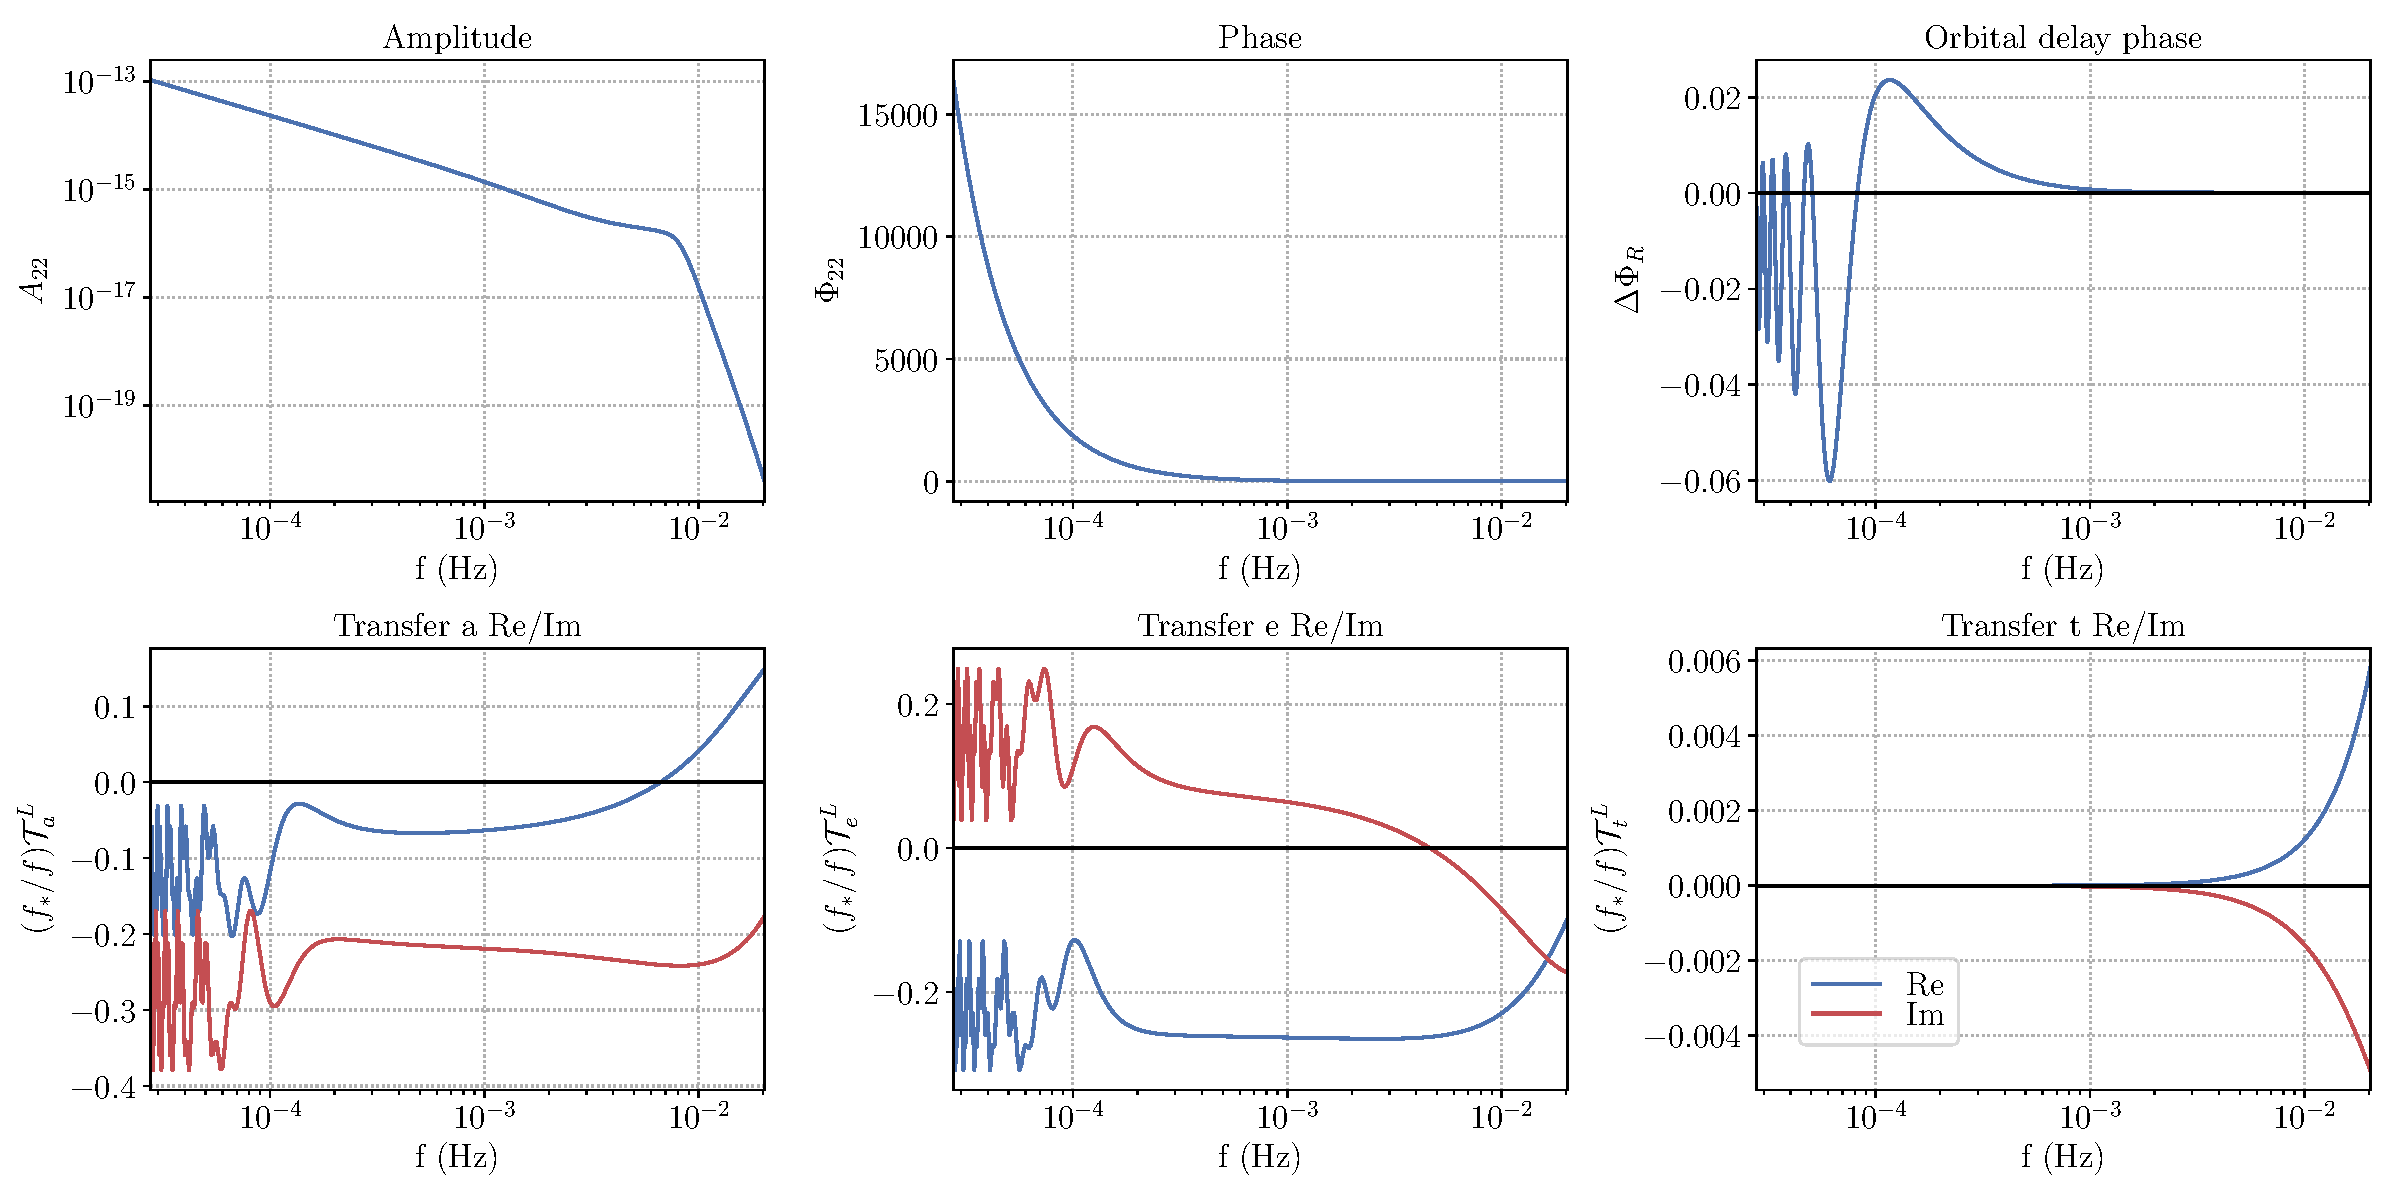
\includegraphics[width=.98\linewidth]{../plots/plot_smbh9_tdi.pdf}
  \caption{\SM{TODO: rethink the visualization, maybe plot only transfer functions}.}
  \label{fig:tranferSMBHCase9}
\end{figure*}

\begin{figure}
  \centering
  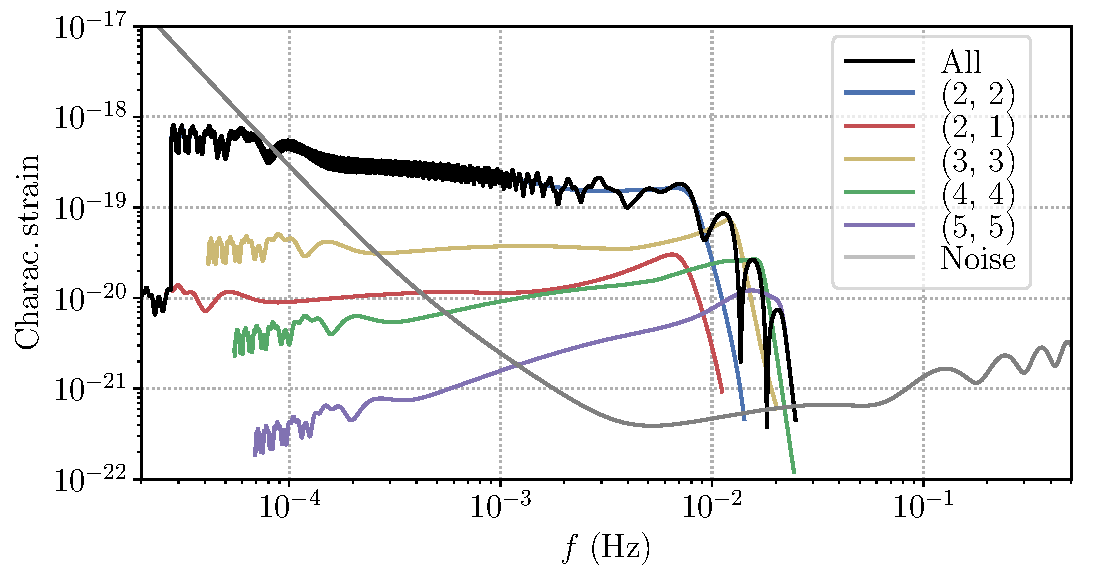
\includegraphics[width=.99\linewidth]{../plots/plot_hc_tdia_hm.pdf}
  \caption{.}
  \label{fig:FDHMSMBHCase9}
\end{figure}

-- add plot for SNR accumulation with time or frequency: inspiral/MRD balance across mass range

%%%%%%%%%%%%%%%%%%%%%%%%%%%%%%%%%%%%

\subsection{Parameter estimation}
\label{sec:SMBHPE}

\begin{figure*}
  \centering
  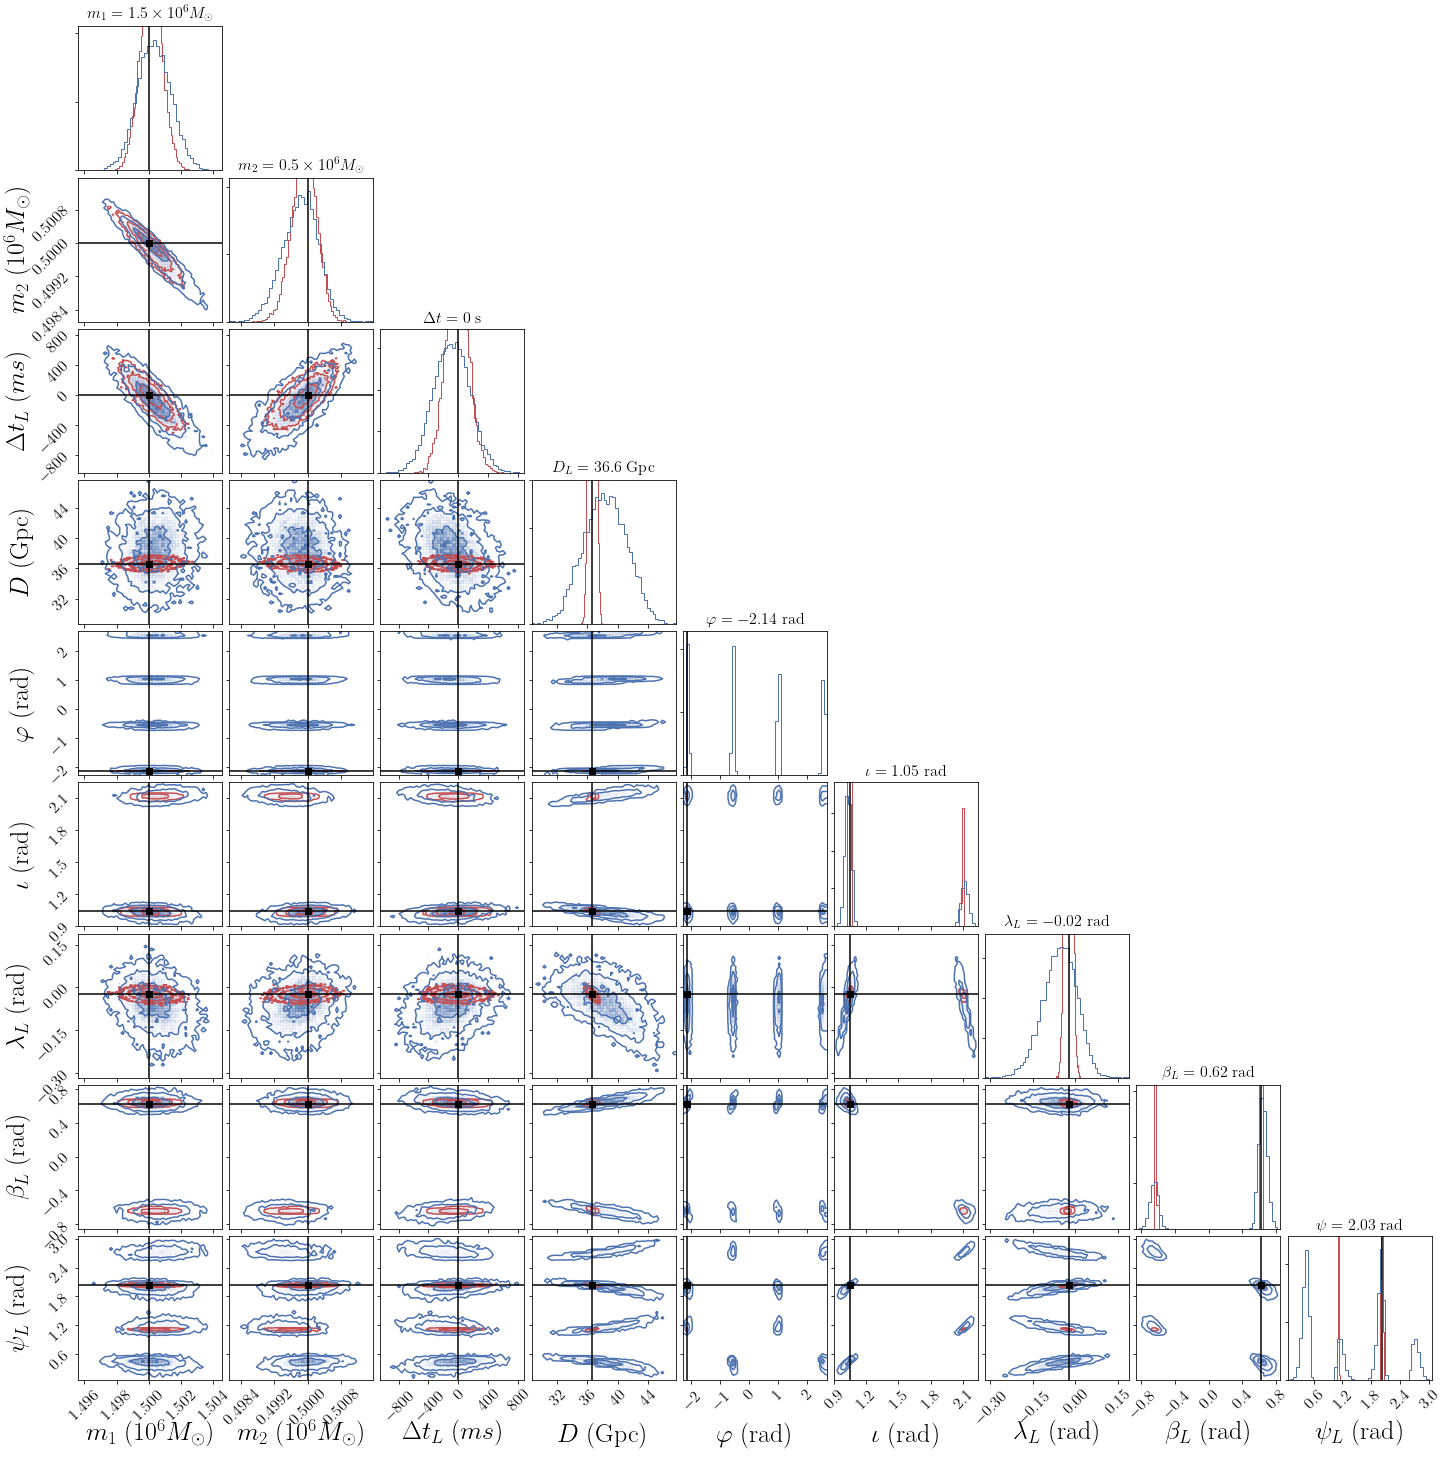
\includegraphics[width=.98\linewidth]{../plots/corner_smbh_case0_ptmcmc_22_hm.png}
  \caption{.}
  \label{fig:PEsmbh22hmCase0}
\end{figure*}

\begin{figure*}
  \centering
  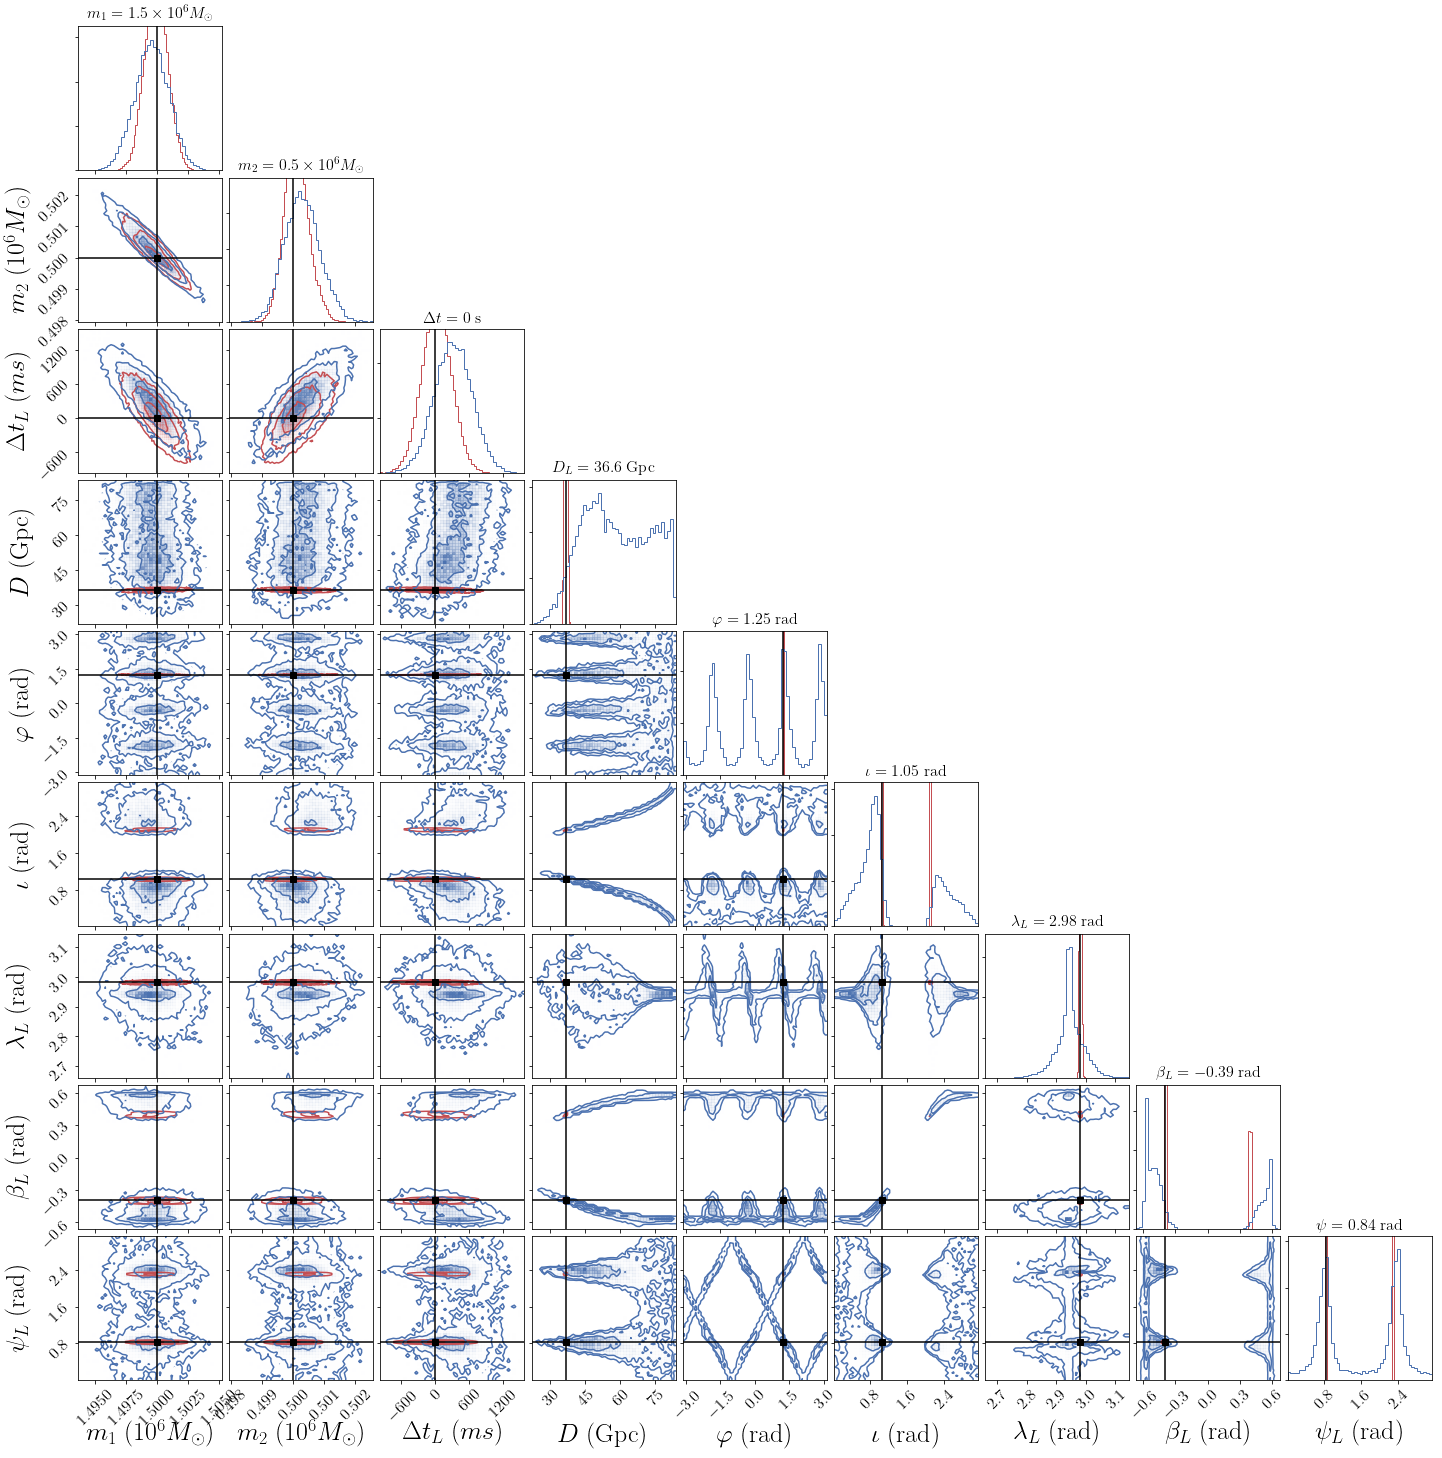
\includegraphics[width=.98\linewidth]{../plots/corner_smbh_case9_ptmcmc_22_hm.png}
  \caption{.}
  \label{fig:PEsmbh22hmCase0}
\end{figure*}

-- High-mass system, non-degenerate, 22 and HM + Fisher - stacked SNR contours
eg:

Case 12?
m1,    m2,    t0,D,     phi0,i,   lam,  bet, psi
8.89e5,1.11e5,0, 3.67e4,pi/3,pi/2,3pi/4,pi/3,pi/3

--enumerate priors

Case 0

-- Performance: waveform and likelihood costs, number of sampler evaluations

%%%%%%%%%%%%%%%%%%%%%%%%%%%%%%%%%%%%

\subsection{Accumulation of signal with time}
\label{sec:SMBHPEacctime}

\begin{figure*}
  \centering
  \begin{minipage}{.32\linewidth}
      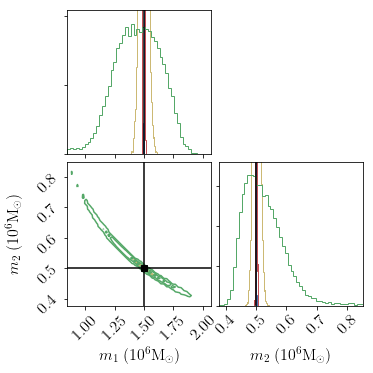
\includegraphics[width=.99\linewidth]{../plots/corner_smbh_case9_hm_tseries_m1m2.png}
   \end{minipage}
   \begin{minipage}{.32\linewidth}
      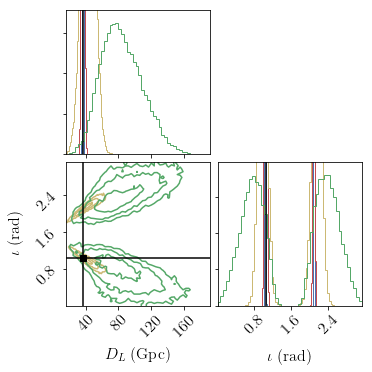
\includegraphics[width=.99\linewidth]{../plots/corner_smbh_case9_hm_tseries_Dinc.png}
   \end{minipage}
   \begin{minipage}{.32\linewidth}
      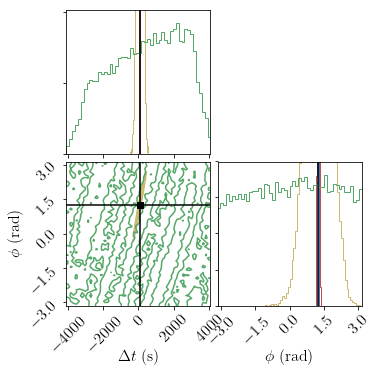
\includegraphics[width=.99\linewidth]{../plots/corner_smbh_case9_hm_tseries_tphi.png}
   \end{minipage}
  \caption{.}
  \label{fig:smbhCornerZoomHMCase9}
\end{figure*}

\begin{figure*}
  \centering
  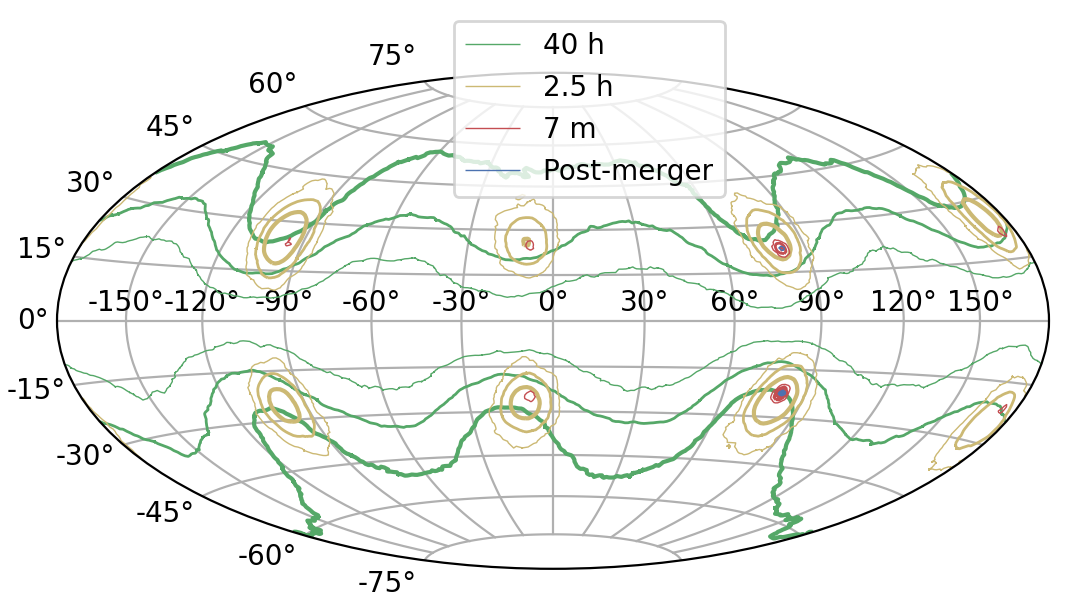
\includegraphics[width=.8\linewidth]{../plots/plot_mollweide_tseries.png}
  \caption{.}
  \label{fig:MollweidesmbhTserieshmCase9}
\end{figure*}

%%%%%%%%%%%%%%%%%%%%%%%%%%%%%%%%%%%%

\subsection{Investigating degeneracies}
\label{subsec:SMBHPEdegen}

\begin{figure*}
  \centering
  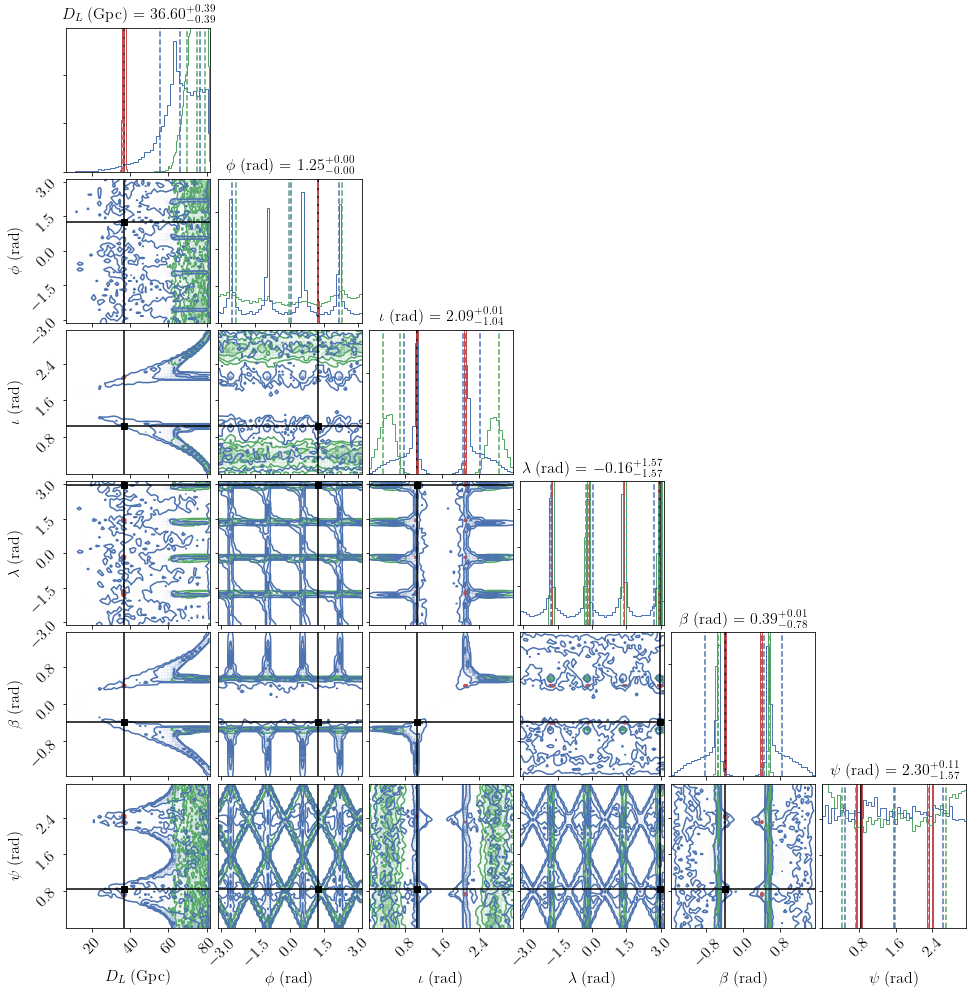
\includegraphics[width=.8\linewidth]{../plots/corner_smbh_case9_simplelike_ptmcmc_bambi.png}
  \caption{Posterior distributions obtained with the two samplers \texttt{PTMCMC} (blue) and $\texttt{MultiNest}$ (green) for the simplified likelihood~\eqref{eq:simplelikelihoodhm}, using only the dominant mode $(\ell, m) = (2,2)$. Masses and time are pinned to the injected value, and the motion of the detector is neglected. We also superimpose (red) the contours obtained with \texttt{MultiNest} by including all harmonics $(2,2)$, $(2,1)$, $(3,3)$, $(4,4)$, $(5,5)$.}
  \label{fig:PEsmbh22hmSimpleLikeCase9}
\end{figure*}

\begin{figure}
  \centering
  \begin{minipage}{.49\linewidth}
  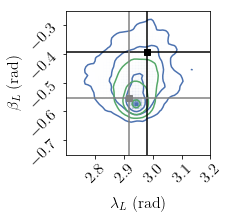
\includegraphics[width=.99\linewidth]{../plots/corner_skydown_smbh_case9_22_ptmcmc_bambi_withdegen.png}
  \end{minipage}
  \begin{minipage}{.49\linewidth}
  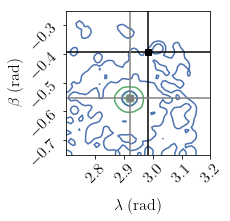
\includegraphics[width=.99\linewidth]{../plots/corner_skydown_smbh_case9_simplelike_ptmcmc_bambi_withdegen.png}
  \end{minipage}
  \caption{Sky position posterior in presence of degeneracies, zooming close to the injected value. The left panel shows the complete likelihood, while the right panel shows the simplified likelihood~\eqref{eq:simplelikelihoodhm} with a motionless LISA and fixed masses and time. The results of \texttt{PTMCMC} (blue) and \texttt{MultiNest} are superimposed. The black cross is the injected value, and the grey cross is the analytic prediction~\eqref{eq:soldegensky} for the offset peak created by degeneracies.}
  \label{fig:Skydownsmbh22hmSimpleLikeCase9}
\end{figure}

In this section, we investigate the cause of the degeneracies appearing in the posterior of Case~II shown in~\ref{subsec:SMBHPE}. Understanding the structure of these features could prove useful to inform Bayesian samplers, for instance by building adapted jump proposal allowing a much faster mixing of MCMC chains than naive methods. a simplified form of the extrinsic likelihood and the structure of its degeneracies.

An important clue about the appearance of these degeneracies is the length of the observable signal. As shown in Fig.~\ref{}, for our example SMBH systems the SNR accumulates in a matter of days before merger, which means that there is only little impact of the modulations caused by the motion of the detector on the TDI transfer functions~\eqref{}. If we can neglect entirely the motion of the detector (which is not quite true as we will see later on), then we are in a regime where the information about the sky position of the source comes essentially from the pattern functions affecting this high-SNR signal. Using the low-frequency approximation (see~\ref{}) and the time-at-LISA $t_{L}$ as a time variable, there is no frequency dependence in the response. A further simplification occurs when pinning the masses and the time of coalescence to their true values. We found indeed that these parameters correlate only weakly to the other ones, so that we can hope to understand the degeneracy features by restricting the analysis to the six extrinsic parameters $(D_{L}, \iota, \varphi, \lambdaL, \betaL, \psiL)$. \TDC{we could make the connection with a similar decoupling in LIGO/Virgo, which is actually what makes low-latency sky localization possible.}

Under all these simplifying assumptions, the likelihood function becomes purely extrinsic, and takes the form of trivial geometric factors multiplying a constant overlap that can be precomputed. Using the subscript $\mathrm{inj}$ for the injected signal, the likelihood~\eqref{eq:defliklihood} is
\be
	\ln \calL = -\frac{1}{2} \left( \tilde{a} - \tilde{a}_{\rm inj} | \tilde{a} - \tilde{a}_{\rm inj} \right) -\frac{1}{2} \left( \tilde{e} - \tilde{e}_{\rm inj} | \tilde{e} - \tilde{e}_{\rm inj} \right) \,.
\ee
From the low-frequency response \eqref{eq:aelowfmodes}, pinning the time-at-LISA~\eqref{} \SM{to be completed for $t_{L}$} so that we can ignore the factor $\exp [2 i \pi f k\cdot p_{0}]$ as a pure constant corresponding to a redefinition of time, we obtain \JGB{Should we use notation $\Phi_R$ here and in \eqref{eq:aelowfmodes}?}
\begin{align}\label{eq:simplelikelihoodhm}
	\ln \calL &= -\frac{1}{2} \sum_{\ell m} \sum_{\ell' m'}   \left[ \left( s_{a}^{\ell m} - s_{a, \mathrm{inj}}^{\ell m}\right) \left( s_{a}^{\ell' m'} - s_{a, \mathrm{inj}}^{\ell' m'}\right)^{*} \right. \nn\\
	& \qquad \left. + \left( s_{e}^{\ell m} - s_{e, \mathrm{inj}}^{\ell m}\right) \left( s_{e}^{\ell' m'} - s_{e, \mathrm{inj}}^{\ell' m'}\right)^{*} \right] \left\langle \ell m | \ell' m' \right\rangle \,,
\end{align}
where we introduced the following extrinsic signal functions \JGB{Since neither $D_{a,e}$ nor $P_{\ell m}$ are defined in the main text, may be better to write in terms of a version of $F$ as in \eqref{eq:defFapcFepc}}
\be\label{eq:defsaelm}
	s_{a,e}^{\ell m} = \frac{1}{d} \frac{2}{3L} D_{a,e} : P_{\ell m} \,,
\ee
with $d = D / D^{\rm inj}$ the dimensionless ratio of luminosity distances. The prefactors $\left\langle \ell m | \ell' m' \right\rangle$ \sout{are pure normalization constants, and} represent mode overlaps as
\be\label{eq:innerproductlmlpmp}
	\left\langle \ell m | \ell' m' \right\rangle = 4\mathrm{Re} \int \frac{df}{S_{n}^{a,e}} \left( 3 \pi f L\right)^{2} \tilde{h}_{\ell m} \tilde{h}_{\ell' m'}^{*} \,.
\ee
Here, the noise PSD $S_{n}^{a,e}$ is given by~\eqref{} and is identical between the channels $a$ and $e$. Having fixed the masses and the time, these overlaps are to be computed with the modes $\tilde{h}_{\ell m}^{\rm inj}$ of the injected signal.

In the case where we only include the dominant harmonic $h_{22}$, the likelihood~\eqref{eq:simplelikelihoodhm} simplifies to
\be\label{eq:simplelikelihood22}
	\ln \calL = -\frac{1}{2} \left\langle 22 | 22 \right\rangle  \left[ \left| s_{a}^{22} - s_{a, \mathrm{inj}}^{22} \right|^{2} + \left| s_{e}^{22} - s_{e, \mathrm{inj}}^{22}\right|^{2} \right] \,.
\ee
The functions~\eqref{eq:defsaelm} take the explicit form
\begin{align}
	s_{a,e}^{22} &= \frac{1}{4d} \sqrt{\frac{5}{\pi}} \cos^{4}\frac{\iota}{2} e^{2i(\varphi-\psiL)} \left( F_{a,e}^{+} + i F_{a,e}^{\times} \right) \\
	&+ \frac{1}{4d} \sqrt{\frac{5}{\pi}} \sin^{4}\frac{\iota}{2} e^{2i(\varphi+\psiL)} \left( F_{a,e}^{+} - i F_{a,e}^{\times} \right) \,,
\end{align}
with the pattern functions for the channels $a$ and $e$ defined in \eqref{eq:defFapcFepc}-\eqref{eq:FapcFepc}.

In order to make more manifest the degeneracies in the problem, it will be useful to introduce the following notations. First, since $\iota \in [0, \pi]$ while $\beta_{L} \in [-\pi/2, \pi/2]$, it will be more convenient to work with $\theta_{L} = \pi/2 - \beta_{L}$. We will further abbreviate notations by using the variables
\TDC{it is unclear if these mean $\tan (\iota/2)$ or $(\tan \iota)/2$}
\be
	t_{\iota} \equiv \tan \frac{\iota}{2} \,, \quad t_{\theta} \equiv \tan \frac{\theta_{L}}{2} \,.
\ee
We also introduce the azimuthal angles $\lambda_{a} = \lambda_{L} - \pi/6$, $\lambda_{e} = \lambda_{L} + \pi/12 = \lambda_{a} + \pi/4$, and form the combinations
\be
	\sigma_{\pm} \equiv s_{a}^{22} \pm i s_{e}^{22} \,.
\ee
In these notations, we obtain
\bsub\label{eq:sigmapm}
\begin{align}
	\sigma_{+} &= \rho e^{2i\varphi} \left[ t_{\theta}^{4} e^{-2 i \psiL} + t_{\iota}^{4} e^{2 i \psiL} \right] e^{-2i \lambda_{a}} \,, \\
	\sigma_{-} &= \rho e^{2i\varphi} \left[ e^{-2 i \psiL} + t_{\theta}^{4} t_{\iota}^{4} e^{2 i \psiL} \right] e^{2i \lambda_{a}} \,,
\end{align}
\esub
with a common prefactor \JGB{This seems to need to  be multiplied by -6 to get what I have in my notes. Trace to change in def of $s_{a,e}$?}
\be\label{eq:sigmafactorrho}
	\rho(d, \iota, \theta_{L}) = \frac{1}{4d} \sqrt{\frac{5}{\pi}} \frac{1}{\left( 1 + t_{\iota}^{2} \right)^{2} \left(1 + t_{\theta}^{2} \right)^{2}} \,.
\ee
Finding points in the parameter space that are degenerate with the injection, i.e. with $\ln \calL \simeq 0$, amounts finding choices for the parameters which obtain the same values for both  $\sigma_{+}$ and $\sigma_{-}$ as the injection.

We can now use the simplified response written in the form~\eqref{eq:sigmapm}-\eqref{eq:sigmafactorrho} to look for symmetries and degeneracies. First, we note the following manifest symmetry: changing simultaneously
\be\label{eq:symmetryresponse}
	\betaL \rightarrow -\betaL\,, \quad \iota \rightarrow \pi - \iota \,, \quad \psiL \rightarrow \pi - \psiL
\ee
leaves the likelihood exactly invariant. There is also a symmetry based on exchanging $\iota \leftrightarrow \theta_{L}$. While leaving $\sigma_-$ unchanged, this conjugates the factor inside brackets for $\sigma_{+}$, which can be compensated using the phase terms $\varphi \pm \lambda_{a}$. If $\Phi = \mathrm{Arg} \left[ t_{\theta}^{4} e^{-2 i \psiL} + t_{\iota}^{4} e^{2 i \psiL} \right]$, we obtain the symmetry
\begin{align}
	\iota' = \theta_{L} \,, \qquad \theta_{L}' = \iota \,, \nn\\
	\varphi' = \varphi + \frac{1}{2} \Phi \quad \mathrm{mod} \; \pi\,, \nn\\
	\lambda_{a}' = \lambda_{a} - \frac{1}{2} \Phi \quad \mathrm{mod} \; \pi\,.
\end{align}

\JGB{Don't have to resort to limits.}
\sout{We can now explain the degenerate features we found as certain limits in this simplified likelihood. In the face-on or face-off limit $\iota \rightarrow 0$, $|t_{\iota}| \ll 1$. This amounts to the $(\ell,m)=(2,2)$ contribution dominating the $(\ell, m)=(2,-2)$ contribution. Neglecting the terms in~\eqref{eq:sigmapm} that are quartic in $t_{\iota}$, we have}
%\bsub\label{eq:sigmapmapprox}
%\begin{align}
%	\sigma_{+} &\simeq \rho e^{2i(\varphi - \psiL)} t_{\theta}^{4} e^{-2i \lambda_{a}} \,, \\
%	\sigma_{-} &\simeq \rho e^{2i(\varphi - \psiL)} e^{2i \lambda_{a}} \,,
%\end{align}
%\esub

Beyond these discrete symetries, since likelihood function dependence on the six extrinsic parameters is funneled through just two complex functions, we should expect a two-dimensional degenerate subspace.  Indeed we can explicitly find a general solution for parameter values that solve $\sigma_{\pm}((D_{L}, t_\iota, t_\theta \varphi, \lambda_a, \psiL)=\sigma_{\pm,{\rm inj}}$, which we just sketch here, as needed to explain features of the degeneracies.

Defining the ratio
\be
	r(\lambda_a, t_\iota, t_\theta, \psiL) = \frac{\sigma_{+}}{\sigma_{-}} \,,
\ee
makes clear that $r=r_{\rm inj}$ provides one complex condition on 4 real unknown parameters, eliminating parameters $D_{L}$ and $\varphi$ while retaining the features of the full degenerate subspace.  Going further, $|r|^2=|r_{\rm inj}|^2$ yields one condition on 3 parameters, eliminating $\lambda_a$.  In fact, with a little rearrangement, this can be written as a quadratic expression for either $t_\iota^4$ or $t_\theta^4$ for an explicit solution.  Depending on the value of $|r_{\rm inj}|^2$, values of $\psiL$ and the independent variable ($t_\theta$ or $t_i$) can always be chosen to guarantee a real, positive solution.

Given a solution for $(t_\iota,t_\theta,\psi_L)$, the rest of the solution then proceeds backwards. An explicit expression for commensurate $\lambda$ comes from solving $r=r_{\rm inj}$, and then $D_L$ and $\varphi$ are obtained from solving, e.g., $s_+=s_{+,{\rm inj}}$.

In the limit that the independent variable is given a value far from unity (near polar $\iota$ ot $\beta_L$), then the solution for the dependent variable approaches a fixed constant special values $t_{\iota,\theta}^4={|r_{\rm inj}|^{\pm1}}$, with leading order corrections proportional to  $t_{\theta,\iota}^{4}$.  A large part of the degenerate subspace volume then tends to found with parameters $\iota$ ot $\beta_L$ near these special values with corresponding constraints on $\lambda$ coming from the solution for the complex argument of $r$.

In terms of the original parameters then, if we consider inferences with the parameter $\iota$ that is not near the source equator, then we find a significant part of the degenerate maximum-likelihood parameter space volume near the special sky positions
\bsub
\begin{align}
  \beta_L&\approx{\beta_L}^{*}=\pm\left(\frac{\pi}{2} - 2 \mathrm{Arctan} \; \left| r_{\rm inj}\right|^{1/4} \right)\,, \\
  \lambda_a&\approx {\lambda_a}^{*}=\frac{\pi}{6} -\frac{1}{4} \mathrm{Arg} \; r_{\rm inj} \;\mathrm{mod}\; \frac{\pi}{2} \,,\\
  \rho e^{2i(\varphi-\psiL)} &\approx e^{-2i\lambda_{a}^{*}} \sigma_{-}^{\rm inj} \,.
\end{align}
\esub
With the $\lambdaL \rightarrow \lambdaL + k \pi/2$ and $\betaL \rightarrow - \betaL$ symmetries, we arrive at eight sky positions where the degeneracy occurs, with an exact degeneracy for the pair of parameters $(\varphi, \psiL)$, as well as an approximate degeneracy for the pair $(d, \iota)$ as long as we remain in the regime $t_{\iota}^{4} \ll 1$ or $t_{\iota}^{4} \gg 1$ (which is quite extended, thanks to the quartic power). For each of these sky positions built from~\eqref{eq:soldegensky}, many different values of $(\varphi, \psiL)$ and $(d, \iota)$ produce a waveform very close to the injection, resulting in apparent peaks in the marginalized posterior distribution for the sky position, located at the special sky positions $(\lambda_{a}^{*}, \theta_{L}^{*})$, which are offset from the injected value.

Without special tuning, the injected sky position which led to the given values of $s_{a,\mathrm{inj}}$ and $s_{e,\mathrm{inj}}$ is correspondingly likely to have been near one of these sky locations, but it may not have been. In those cases the posterior\ldots

Similarly, considering inferred locations away from the LISA-constellation plane, we find a significant part of the degenerate parameter space near special values for inclination and correspondingly for $\lambda_L+\varphi$
\bsub
\begin{align}
	\iota&\approx\iota^{*} = 2 \mathrm{Arctan} \; \left| r_{\rm inj}\right|^{1/4} \,, \\
	\lambda_a-\psiL&\approx (\lambda_{a} - \psiL)^{*} = -\frac{1}{4} \mathrm{Arg} \; r_{\rm inj} \;\mathrm{mod}\; \frac{\pi}{2} \,\\
        \rho e^{2i\varphi} &\approx e^{-2i (\lambda_{a} - \psi_{L})^{*}} \sigma_{-}^{\rm inj} \,.
\end{align}
\esub



%finding $(\lambda_{a}^{*}, \theta_{L}^{*})$ verifying
%\be\label{eq:degenconditionsky}
%	\frac{\sigma_{+}}{\sigma_{-}} (\lambda_{a}^{*}, \theta_{L}^{*}) = r_{\rm inj} \,,
%\ee
%with the approximation~\eqref{eq:sigmapmapprox} for the left-hand side, guarantees that we can then match both $\sigma_{+}$ and $\sigma_{-}$ of the injection with the condition
%\be\label{eq:degenconditionprefactor}
%	\rho e^{2i(\varphi - \psiL)} e^{2i \lambda_{a}^{*}} = \sigma_{-}^{\rm inj}\,.
%\ee
%In the limit $|t_{\iota}| \ll 1$,
%\be
%	\frac{\sigma_{+}}{\sigma_{-}} \simeq t_{\theta}^{4} e^{-4i\lambda_{a}} \,,
%\ee
%so that~\eqref{eq:degenconditionsky} is verified for special positions in the sky at (coming back to the original variables $(\lambdaL, \betaL)$)
%\bsub\label{eq:soldegensky}
%\begin{align}
%\beta_{L}^{*} &= \frac{\pi}{2} - 2 \mathrm{Arctan} \; \left| r_{\rm inj}\right|^{1/4} \,, \\
%	\lambda_{L}^{*} &= \frac{\pi}{6} -\frac{1}{4} \mathrm{Arg} \; r_{\rm inj} \;\mathrm{mod}\; \frac{\pi}{2} \,.
%\end{align}
%\esub
\JGB{Keep something from this?}
The other condition~\eqref{eq:conditionprefactor} gives then a single phase constraint for $\varphi - \psiL$, and a single amplitude constraint for $\rho(d, \iota, \theta_{L}^{*})$. The limit $\iota \rightarrow \pi$ (where the $(2,-2)$ contribution dominates the $(2,2)$) is very similar, as can be seen most easily by the change of variable $\iota \rightarrow \pi - \iota$, with $-\psiL$ and $\pi - \theta_{L}$ playing the roles of $\psiL$ and $\theta_{L}$.


%We can further find the same mechanism, with a few differences, by exchanging the roles of $(\iota, \varphi)$ and $(\theta_{L}, \lambda_{a})$, as follows. In the limit $\theta_{L} \rightarrow 0$ with $|t_{\theta}| \ll 1$, we have this time
%\be
%	\frac{\sigma_{+}}{\sigma_{-}} \simeq t_{\iota}^{4} e^{-4i(\lambda_{a} - \psi_{L})} \,,
%\ee
%which gives in the same way a degeneracy if
%\bsub\label{eq:soldegeniotaphi}
%\begin{align}
%	\iota^{*} &= 2 \mathrm{Arctan} \; \left| r_{\rm inj}\right|^{1/4} \,, \\
%	(\lambda_{a} - \psiL)^{*} &= -\frac{1}{4} \mathrm{Arg} \; r_{\rm inj} \;\mathrm{mod}\; \frac{\pi}{2} \,,
%\end{align}
%\esub
%with a condition on $\rho$ and $\varphi$ that is now
%\be
%\rho e^{2i\varphi} e^{2i (\lambda_{a}^{*} - \psi_{L}^{*})} = \sigma_{-}^{\rm inj} \,.
%\ee
\JGB{Keep something from this?}
Thus, we find again a degenerate pattern, with the difference that \eqref{eq:soldegeniotaphi} imposes a condition on the pair $\lambda_{a} - \psiL$ instead of $\lambda_{a}$, and the extra condition imposes a condition on $\varphi$ instead of the pair $\varphi - \psiL$.

When considering more harmonics beyond the dominant mode $h_{22}$, such degeneracies will be broken easily. As in the case of the full likelihood, the simplified likelihood~\eqref{eq:simplelikelihoodhm} will have several terms with different inclination and phase dependencies. If the signal is loud enough for at least two modes to be detected, then the inclination $\iota$ and the phase $\varphi$ are fixed by the relative amplitude and phase of these modes. This will break the degeneracies $(d, \iota)$ and the degeneracy $(\varphi, \psiL)$.

We illustrate our findings by running a Bayesian parameter estimation for the simplified likelihood~\eqref{eq:simplelikelihood22} with the two samplers \texttt{MultiNest} and \texttt{PTMCMC} described in Sec.~\ref{}. Since the inner products~\eqref{eq:innerproductlmlpmp} are constants computed only once, the external factors become trivially inexpensive, and the likelihood is very fast to compute. We take advantage of this to run \texttt{PTMCMC} for a very large number of steps, ensuring that we do not miss degenerate regions of the parameter space. The resulting posterior distribution is extremely degenerate, as shown in Fig.~\ref{fig:PEsmbh22hmSimpleLikeCase9}. The sampler \texttt{MultiNest} fails to resolve this structure, stopping after having only explored the degenerate region $\iota \rightarrow 0$ and $\iota \rightarrow \pi$ and the eight sky positions~\eqref{eq:soldegensky}. In accordance with~\eqref{eq:degenconditionsky}-\eqref{eq:degenconditionprefactor}, this corresponds to lines in $\varphi \pm \psiL = \mathrm{const}$. The sampler \texttt{PTMCMC} finds more degenerate regions, in particular it finds similar structures with the roles of $\iota$ and $\betaL$ exchanged (as shown notably by the $(d,\iota)$ and $(d,\betaL)$ panels), as well as intermediate regions connecting all these features.

Fig.~\ref{fig:PEsmbh22hmSimpleLikeCase9} also shows the result obtained when including all available harmonics~\eqref{} in~\eqref{eq:simplelikelihoodhm}. The degenerate structures collapse to leave only eight modes corresponding to $\betaL \rightarrow - \betaL$ and $\lambdaL \rightarrow \lambdaL + k\pi/2$. We found that this degeneracy-breaking occurs already when including a single subdominant harmonic $h_{21}$.

We can now come back to explaining the results of Sec.~\ref{}, and in particular Fig.~\ref{}, obtained with the true likelihood function for the mode $h_{22}$. First, the difference between the two Bayesian samplers has been made more extreme by going to the more degenerate likelihood~\eqref{eq:simplelikelihood22}, allowing us to attribute their disagreement to an apparent shortcoming of \texttt{MultiNest}\footnote{We recall that we only used standard values for the metaparameters \SM{[complete]} for this sampler, and we do not exclude that it would be possible to improve results with minor changes.} for resolving extended degenerate regions. Focusing on the sky position, we zoom close to the injection in Fig.~\ref{fig:Skydownsmbh22hmSimpleLikeCase9}. We compare here the posterior distribution generated with the true likelihood with the one obtained with the simplified likelihood~\eqref{eq:simplelikelihood22}, for both samplers.  We also superimpose the prediction~\eqref{eq:soldegensky} for the degeneracy-induced peak. We see that, although ,

%\be\label{eq:symmetryresponse}
%\betaL \rightarrow -\betaL\,, \quad \iota \rightarrow \pi - \iota \,, \quad \psiL \rightarrow \pi - \psiL
%\ee
%leaves the signal unchanged. We can also rewrite the likelihood in a way that makes clearer the symmetry between the two pairs of parameters $(\iota, \varphiL)$ and $(\betaL, \lambdaL)$ \SM{[TODO]}.
%
%The simplified extrinsic likelihood for a frozen LISA then takes the form
%\be\label{eq:simplelikelihood}
%	\ln \calL = - \frac{1}{2} \Lambda \left( \left| s_{a} - s_{a}^{\rm inj} \right|^{2} + \left| s_{e} - s_{e}^{\rm inj} \right|^{2} \right) \,,
%\ee
%where $\Lambda$ appears as an overall normalization factor, playing the role of the square SNR of the signal.

%We can now explore possible degeneracies in the likelihood given by~\eqref{eq:simplelikelihood}, \eqref{eq:defsase} and \eqref{eq:defa22a2m2}-\eqref{eq:defe22e2m2}. We note that the relative contributions of the modes $h_{2,2}$ and $h_{2,-2}$ are strongly separated in the face-on or face-off limit, leading to a simplification of the response and an enhanced degeneracy. Due to the symmetry~\eqref{eq:symmetryresponse}, we will focus on the face-on limit $\iota \rightarrow 0$. In this limit, the $h_{2,-2}$ contributions die off rapidly as $a_{2,-2}\,, e_{2,-2} \sim \sin^{4} (\iota/2)$. If they are assumed to be negligible, then we can rewrite
%\bsub\label{eq:saseapprox}
%\begin{align}
%	s_{a} \simeq i\calA e^{2 i \xi} \left( D_{a}^{+} + i D_{a}^{\times} \right) \,, \\
%	s_{e} \simeq i\calA e^{2 i \xi} \left( D_{e}^{+} + i D_{e}^{\times} \right) \,,
%\end{align}
%\esub
%where we introduced the notations $\xi (\varphiL, \psiL) \equiv -\varphiL - \psiL$ and $\calA(d, \iota) \equiv 3/4\sqrt{5/\pi}\cos^{4}(\iota/2)/d $ for the common phase and amplitude factors.
%
%For a degeneracy to occur, both complex quantities $s_{a}$ and $s_{e}$ must be close to the injection values $s_{a}^{\rm inj}$ and $s_{e}^{\rm inj}$, which can be achieved as follows if~\eqref{eq:saseapprox} is valid. Defining the complex ratio
%\be\label{eq:defr}
%	r(\lambdaL, \betaL) = \frac{D_{a}^{+} + i D_{a}^{\times}}{D_{e}^{+} + i D_{e}^{\times} } \,,
%\ee
%if the position in the sky $(\lambda_{L}^{*}, \beta_{L}^{*})$ can be chosen so that
%\be\label{eq:rcondition}
%	r(\lambda_{L}^{*}, \beta_{L}^{*}) = \frac{s_{a}^{\rm inj}}{s_{e}^{\rm inj}} \,,
%\ee
%then adjusting $\calA$ and $\xi$ so that
%\be
%	i\calA e^{2 i \xi} = \frac{s_{a}^{\rm inj}}{\left( D_{a}^{+} + i D_{a}^{\times} \right)(\lambda_{L}^{*}, \beta_{L}^{*})}
%\ee
%generates degenerate points in parameter space with $\ln \calL \simeq 0$.
%
%The conditions~\eqref{eq:defr}-\eqref{eq:rcondition} can be inverted for the sky position as follows. For a given complex value of $r = s_{a}^{\rm inj} / s_{e}^{\rm inj}$, $r(\lambda_{L}^{*}, \beta_{L}^{*}) = r$ can be rewritten as
%\be\label{eq:eqtosolveforlambdabetaL}
%	e^{4i\lambda_{L}^{*}}e^{i\frac{\pi}{3}} \frac{\left( 1 +\sin\beta_{L}^{*} \right)^{2}}{\left( 1 - \sin\beta_{L}^{*} \right)^{2}} = \frac{1+ i r}{1 - i r} \,.
%\ee
%Solving for the modulus of~\eqref{eq:eqtosolveforlambdabetaL} then yields
%\be\label{eq:solutionbetaL}
%	\sin\beta_{L}^{*} = \frac{\rho - 1}{\rho + 1} \,,
%\ee
%for
%\be
%	\rho = \sqrt{\left| \frac{1+ i r}{1 - i r} \right|} \,.
%\ee
%Solving for the argument of~\eqref{eq:eqtosolveforlambdabetaL} gives four solutions for $\lambda_{L}^{*}$ as
%\be\label{eq:solutionlambdaL}
%	\lambda_{L}^{*} = - \frac{\pi}{12} + \frac{1}{4}\mathrm{Arg} \frac{1+ i r}{1 - i r} + \frac{k \pi}{2} \quad \mathrm{for} \quad k = 0,\dots,3 \,.
%\ee
%
%Repeating the argument for the other branch of solutions $\iota \rightarrow \pi$ (or directly considering the symmery~\eqref{eq:symmetryresponse}) gives four other solutions in the sky with identical sky longitudes $\lambda_{L}^{*}$, with symmetrized sky latitudes $\beta_{L}^{*} \rightarrow -\beta_{L}^{*}$, and with $\xi (\varphiL, \psiL) \equiv -\varphiL + \psiL$, $\calA(d, \iota) \equiv 3/4\sqrt{5/\pi}\sin^{4}(\iota/2)/d $.
%
%Thus, with~\eqref{eq:solutionbetaL}, \eqref{eq:solutionlambdaL} and $\beta_{L}^{*} \rightarrow -\beta_{L}^{*}$, we arrive at eight degenerate positions in the sky $(\lambda_{L}^{*}, \beta_{L}^{*})$. For each of these sky positions, an exact line degeneracy exists between $\varphiL$ and $\psiL$ as long as $\xi = \mathrm{const}$, as well as an approximate line degeneracy between $d$ and $\iota$, as long as $\calA = \mathrm{const}$, limited to inclination values where $\sin^{4}(\iota/2)$ (or $\cos^{4}(\iota/2)$, for the other branch of solutions) remains negligible. The combination of these degeneracies generates an extended structure in the multi-dimensional parameter space. As a result, when considering the marginal posterior for the sky position, these degenerate spots in the sky can have a lot of probability support.


%%%%%%%%%%%%%%%%%%%%%%%%%%%%%%%%%%%%
\section{Stellar origin black holes}
\label{sec:SOBH}

-- SOBH system, SNR sufficient for clean analysis + Fisher - stacked SNR contours
-- Performance: waveform and likelihood costs, number of sampler evaluations

Stellar-origin black-hole (SOBH) mergers have been recently recognized as an
important source of LISA detections \cite{Sesana16} although full parameter
estimation studies are not available yet. In this section we present two case
studies of parameter inference for such sources using the formalism and methods
described earlier. The parameters of the simulated mergers are taken from the
Radler LISA data challenge and are listed in Table \ref{table:sobh_params}.
\begin{table}
	\begin{tabular}{|c||c|c|}
		\hline
		Radler entry 		& 1 	& 12   \\
		\hline
		Mass 1 ($\Msol$) 	& 21.4	& 63.5 \\
		\hline
		Mass 2 ($\Msol$) 	& 20.1	& 45.1 \\
		\hline
		Distance (Mpc) 		& 49.1	& 318  \\
		\hline
		LISA SNR 			& 26.6	& 11.9 \\
		\hline
	\end{tabular}
	\caption{Parameters of the simulated SOBH mergers. \TDC{Maybe we can show
			 these on the upper right of each corner plot instead.}}
	\label{table:sobh_params}
\end{table}

We caution the reader that our purpose here is to show the feasibility of
Bayesian inference for SOBH sources in LISA using the methodology presented in
this paper. It is by no means a final answer on how to do so in an optimal or
convenient way.  For this reason, the problem is posed in a simplified
way here: in particular, the SOBH signal is assumed to merge roughly at the end of
the observation epoch, and the finite observation time is enforced by
converting it to a minimum analyzed Fourier frequency via the time-frequency
relation of a simple Newtonian inspiral. In a more realistic situation, the
merger time would likely be free to range from the beginning of the observation
to years after its end, and the frequency of the signal at the beginning of the
observation would be another sampling parameter.

The waveform model used to work with SOBH systems is the same phenomenological
approximant \texttt{EOBNRv2HMROM} used earlier, extended at low frequency with a post-Newtonian
frequency-domain waveform. In practice, because LISA only observes the early
inspiral of SOBH systems, only the post-Newtonian waveform plays a role here.
We do not expect radiation modes beyond the quadrupole to give a significant
contribution to the parameter estimates, so we only include the $(2,2)$ mode
for simplicity. We do not include any effect arising from black-hole spins.

As done in the previous section, we apply our parameter inference procedure to
these systems using both BAMBI and parallel-tempered MCMC sampling, and we
numerically evaluate the Fisher matrix at the parameters of the injection.

Due to the duration of an SOBH inspiral in the LISA band, and the complete lack
of merger and ringdown, the chirp mass $\Mchirp$ is measured much better than
other mass parameters and the component masses have a much stronger correlation
than usually found with ground-based gravitational-wave detectors. In order for
the sampling to converge robustly in a reasonable time, we find it is necessary
to express the mass parameters in terms of $\Mchirp$ and symmetric mass ratio
$\eta$, and a relatively tight prior around the injected parameters is required
as well.

In order to generate these results, our PTMCMC sampler requires between
$5\times 10^5$ and $3\times 10^6$ steps with 100 temperatures, taking on the
order of days on a single CPU core without careful optimization. The BAMBI
sampling, on the other hand, completes in tens of minutes only.

The resulting posterior distributions are shown in Fig.~\ref{fig:sobh_corner_1}
and \ref{fig:sobh_corner_12}. We find close agreement between the BAMBI and
PTMCMC samplers. The full joint distributions are fairly complex, but the
complexity is mostly restricted to multimodalities and degeneracies in the
angular parameters only. The typical degeneracy between inclination and distance
is evident. Masses, merger time, distance, inclination and sky location, which
are arguably the most astrophysically useful parameters, have simple marginal
distributions with a well-defined mode and close to Gaussian, even at these
moderate SNR values. The Fisher matrix estimates represent the marginal
distributions of these parameters at least to the order of magnitude. In some
cases the Fisher estimates approximate very precisely even the joint
distributions of pairs of these parameters.

\begin{figure*}
	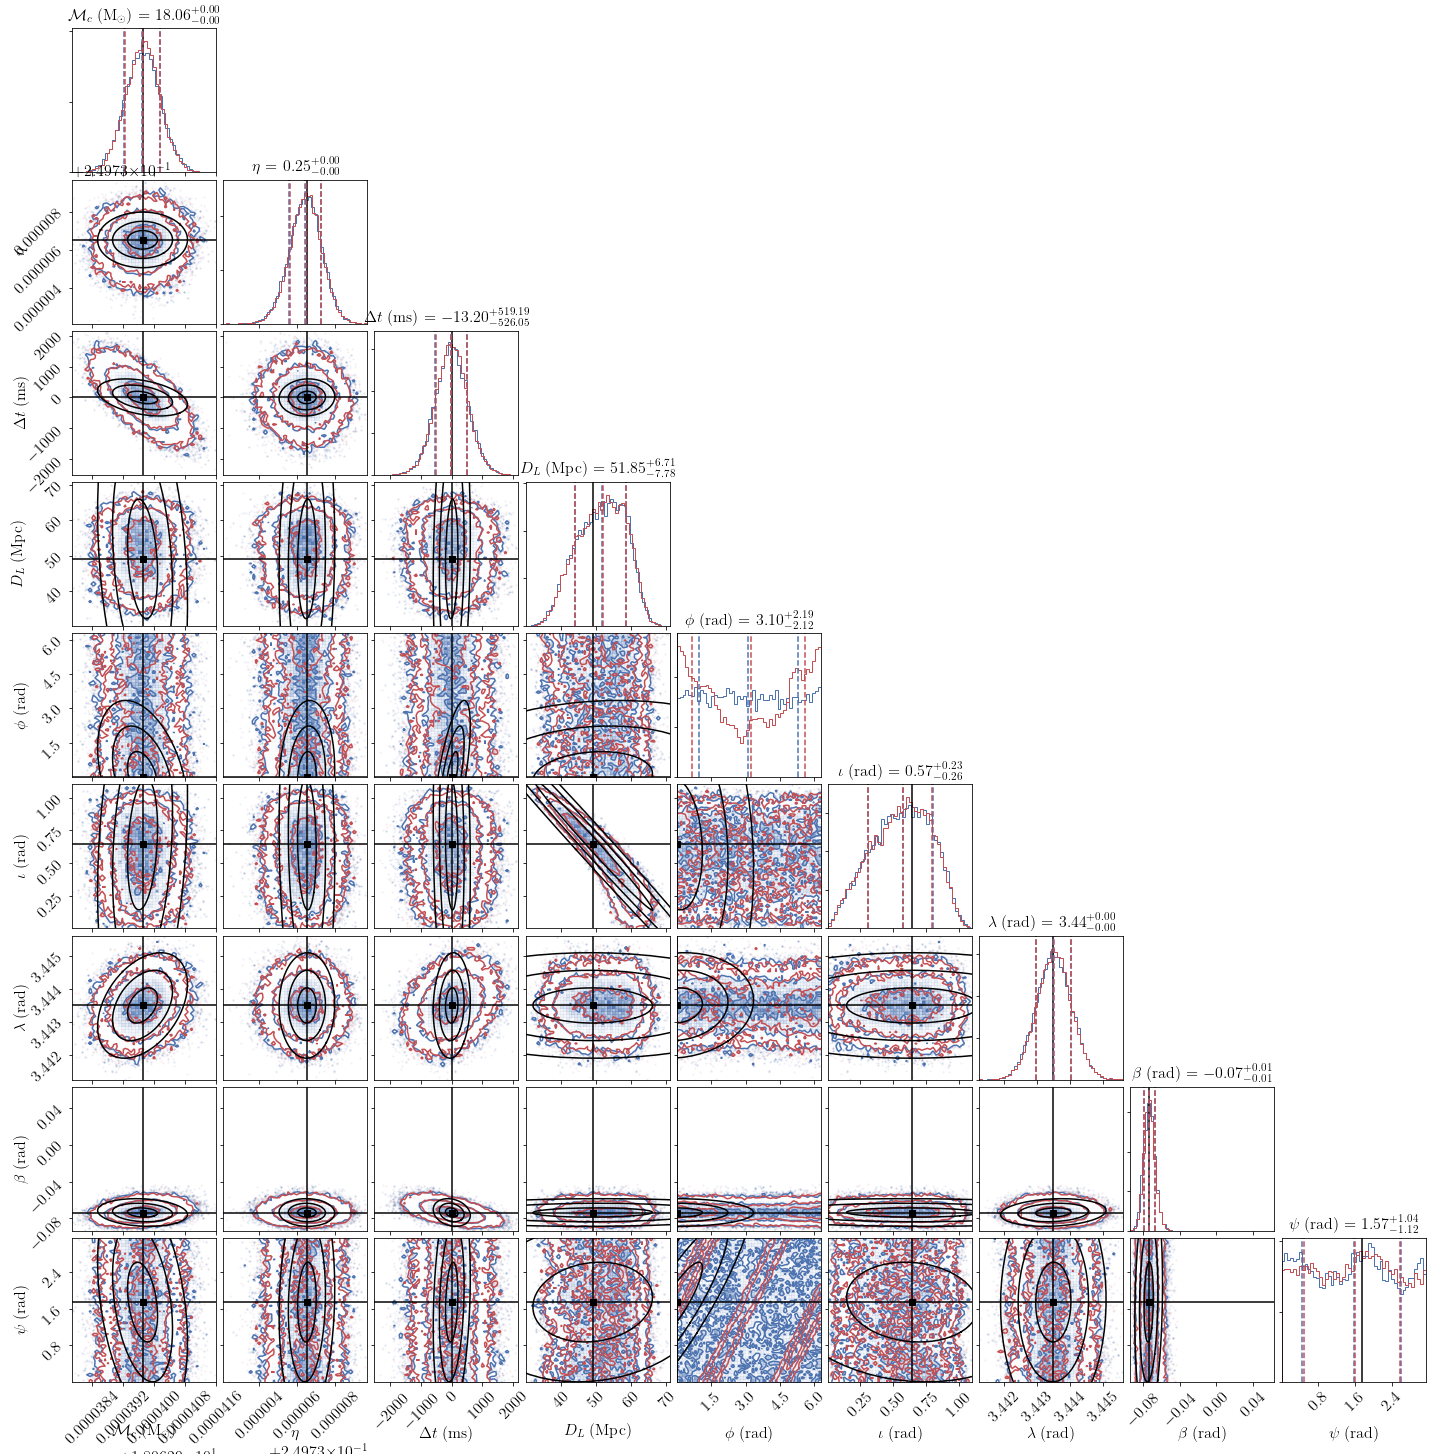
\includegraphics[width=\textwidth]{../plots/corner_sobh_tdc1_ptmcmc_bambi}
	\caption{Inferred parameter posterior distribution for SOBH system 1.}
	\label{fig:sobh_corner_1}
\end{figure*}

\begin{figure*}
	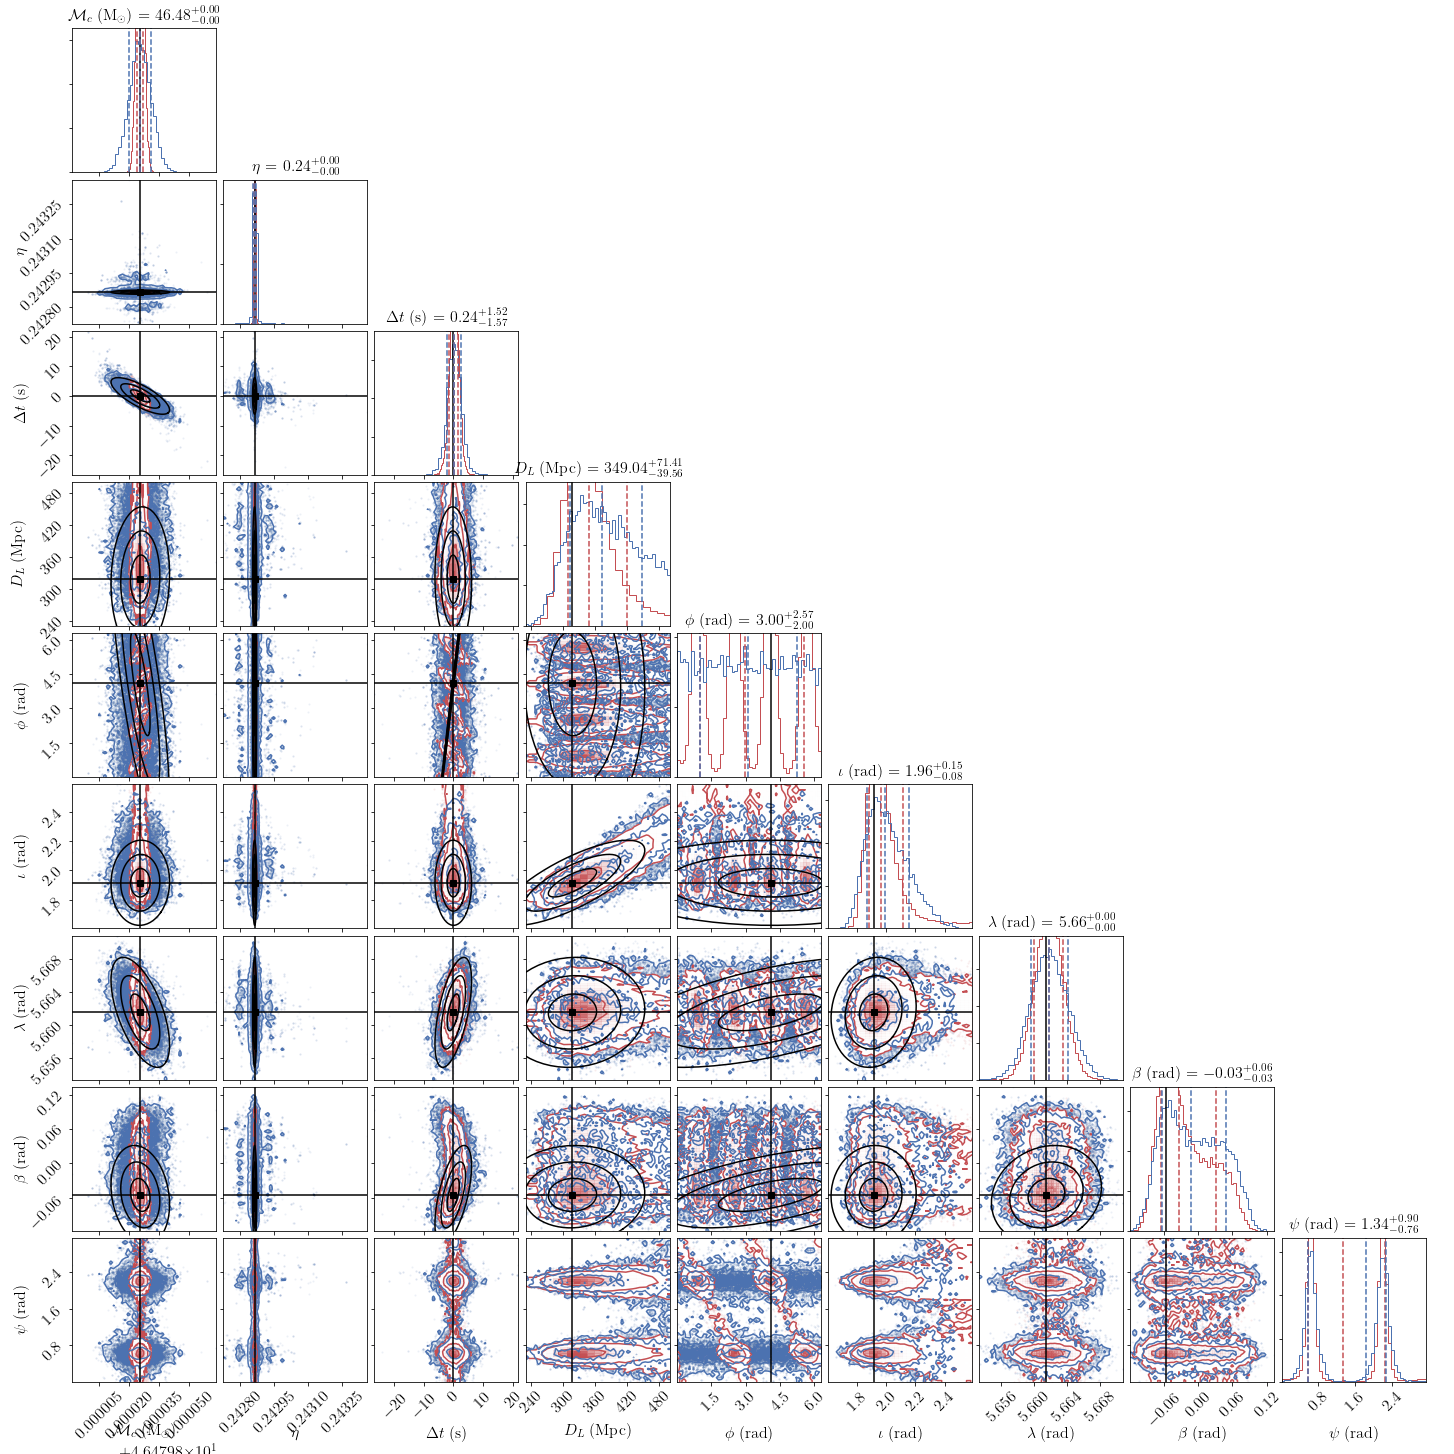
\includegraphics[width=\textwidth]{../plots/corner_sobh_tdc2_ptmcmc_bambi}
	\caption{Inferred parameter posterior distribution for SOBH system 12.}
	\label{fig:sobh_corner_12}
\end{figure*}

Such posterior distributions should not be taken literally as expectations of
LISA's capability for SOBH systems. One reason is the simplified treatment of
the finite observation time described earlier. A second reason is the assumption
of zero black-hole spins, which artificially reduces the width of the posterior
distribution due to the strong degeneracy between spins and symmetric mass
ratio \cite{Baird+2013}.

%%%%%%%%%%%%%%%%%%%%%%%%%%%%%%%%%%%%

\subsection{Signals and transfer functions}
\label{subsec:signaltransferSOBH}

\begin{figure*}
  \centering
  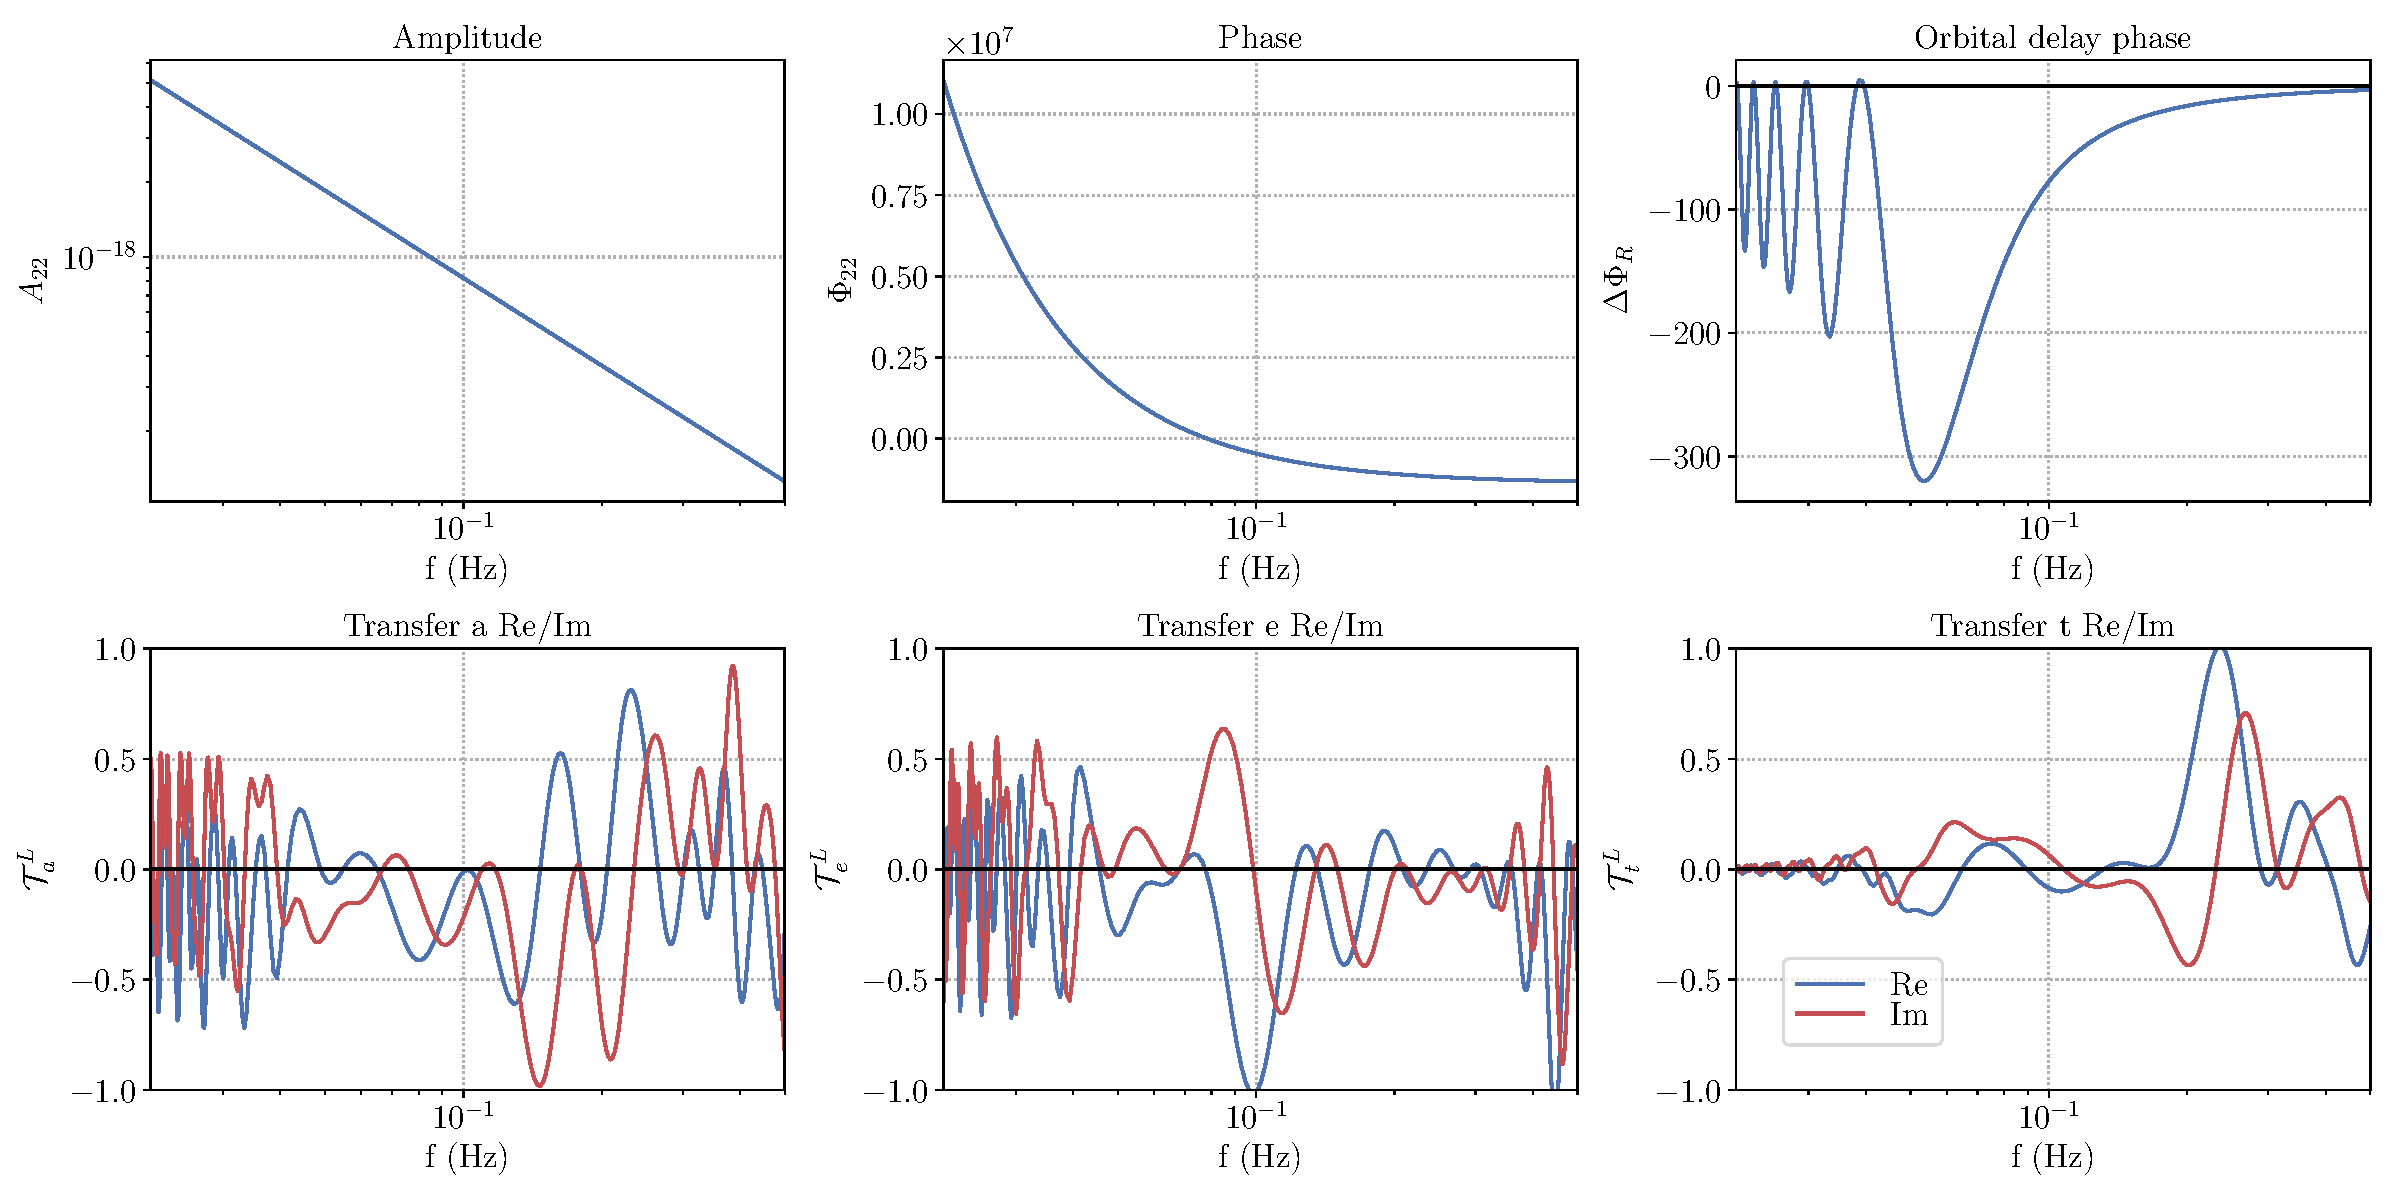
\includegraphics[width=.98\linewidth]{../plots/plot_sobh1_tdi.pdf}
  \caption{\SM{TODO: rethink the visualization, maybe plot only transfer functions}.}
  \label{fig:PEsmbh22hmCase0}
\end{figure*}

%%%%%%%%%%%%%%%%%%%%%%%%%%%%%%%%%%%%
%%%%%%%%%%%%%%%%%%%%%%%%%%%%%%%%%%%%

\section{Discussion}
\label{sec:discussion}

- Summary/conclusions


----------------
Other questions:
- special orientations/sky locations ?
- Fisher matrix qualification - explore parameter choices
- continuously increase SNR - include on these examples
- continuously accumulate information over time
- full exploration of parameter space for all of the above...


%%%%%%%%%%%%%%%%%%%%%%%%%%%%%%%%%%%%
%%%%%%%%%%%%%%%%%%%%%%%%%%%%%%%%%%%%

\appendix

%%%%%%%%%%%%%%%%%%%%%%%%%%%%%%%%%%%%
%%%%%%%%%%%%%%%%%%%%%%%%%%%%%%%%%%%%

\section{The LISA instrument response}
\label{app:response}

%%%%%%%%%%%%%%%%%%%%%%%%%%%%%%%%%%%%%
%
%\subsection{The LISA response - OLD}
%\label{sec:lisaresponse}
%
%\SM{------------------------------------------------------}
%
%\SM{[copy-paste from previous paper -- just here to copy needed formulas / refs]}
%
%We begin by detailing the model that we use for the response of a LISA-like detector, together with the assumptions used and their limitations. Since our aim is to assess the accuracy of our direct Fourier-domain treatment of the response, we can focus on the gravitational-wave contribution to the basic single-link observables. We therefore use a somewhat simplified model for the time-domain response~\cite{Krolak+04}, ignoring corrections that would be crucial from the point of view of noise cancellations, keeping in mind that the response model can be enriched later without affecting the conclusions of the present analysis.
%
%The frequency-shift response for a single link~\eqref{eq:yslr} was derived in Ref.~\cite{EW75} (see also~\cite{CR02, RCP04, Finn08, Cornish09}). Several assumptions enter the result as written in~\eqref{eq:yslr}: (i) effects of the order $v/c$ are neglected, including for instance the special relativistic Doppler effect created by the relative speeds of the spacecraft on their orbits (ii) the propagation is assumed to take place in a flat spacetime, perturbed only by the gravitational wave; thus the gravitational redshift as well as the deflection of light created by the gravitational potential of the Sun is ignored (iii) all geometric factors are evaluated at a single time, whereas one should consider the beam as propagating from the position of the first spacecraft at the time of emission to the position of the second scapecraft at the time of reception, leading to a point-ahead effect.
%
%Additionally, we limit ourselves to a rigid model for the orbits of the constellation, namely we assume that the constellation remains in an equilateral configuration with fixed armlengths. These simplified orbits neglect (iv) effects of order $e^{2}$ from the eccentricity of the individual Keplerian orbits, (v) the effect of gravitational perturbations coming from other celestial bodies, such as the Earth, the quadrupole of the Sun, and the other planets. Note that although we can neglect all the effects (i)-(v) for our present study, keeping track of these corrections is crucial for the purpose of laser noise cancellations, and led to the development of new generations of TDI observables~\cite{Tintoliving}.
%
%It is natural to split the response~\eqref{eq:yslr} into two steps: first the orbital delay related to the orbit around the Sun of the whole constellation, and then the constellation response. The baselines for the delays are indeed very different in the two cases. Geometrical projection factors aside, we have for the orbit around the Sun $R=1\text{au}=1.5\times 10^{8} \text{km}$, while the detector armlength is $L=2.5\times 10^{6}\text{km}$ (in the configuration proposed in~\cite{LISA17}). It is natural to define two transfer frequencies for the two relevant length scales for the delays, defined such that a wavelength fits within this length scale, i.e. $2\pi f d = 1$. This gives
%\begin{subequations}\label{eq:transferfrequencies}
%\begin{align}
%	f_{R} &= 3.2\times10^{-4}\Hz \,,\\
%	f_{L} &= 1.9\times 10^{-2}\Hz \,.
%\end{align}
%\end{subequations}
%The LISA response will behave qualitatively differently on the three frequency bands $f \leq f_{R}$, $f_{R} \leq f \leq f_{L}$ and $f_{L} \leq f$.
%
%The first stage of the response, the orbital delay, consists simply in applying the varying time delay to bring the wavefront sampling point from the SSB reference to the center of the LISA triangular constellation, common to all $y_{slr}$ observables. For $h^{\rm TT}$ the transverse-traceless gravitational waveform in matrix form, we write this orbital time delay as
%\be\label{eq:defresponse0}
%	h_{0}^{\rm TT} (t) = h^{\rm TT}(t-\hatk\cdot p_{0}) \,,
%\ee
%with $p_{0}$ the position of the constellation center, which follows the Earth orbit around the Sun. The second stage of the response calculation comprises the remaining, constellation-centered response. For the single-link contribution to the response, for the laser link from spacecraft $s$ to spacecraft $r$ along a path in direction $n_l$, we write
%\begin{align}\label{eq:defresponseL}
%	y_{slr} &= \frac{1}{2} \frac{1}{1 - \hatk\cdot n_{l}} \nn\\
%	& \cdot n_{l}\cdot \left[ h_{0}^{\rm TT}(t - L - \hatk\cdot p^{L}_{s}) - h_{0}^{\rm TT}(t - \hatk\cdot p^{L}_{r}) \right] \cdot n_{l}\,,
%\end{align}
%where we reference the positions of the spacecraft relative to the center of the constellation, $p^{L}_{A} \equiv p_{A} - p_{0}$.
%
%As described in App.~\ref{app:notation} We will decompose the full signal in the contributions of the individual spin-weighted spherical modes $h_{\ell m}$, whose Fourier transforms are assumed to have a smooth amplitude and phase. First, we define the matrices $P_{+},P_{\times}$ such that, in the sense of matrices,
%\be
%	h^{\rm TT} = h_{+}P_{+} + h_{\times}P_{\times} \,.
%\ee
%We focus only on positive frequencies. Assuming that the approximation~\eqref{eq:zeronegativef} applies, we consider a single mode contribution, $h=h_{\ell m}$ with $m>0$. For each given mode we define a complex matrix $P_{\ell m}$ incorporating the spin-weighted spherical harmonic constant factor as
%\be
%	P_{\ell m} =
%	\begin{cases}
%	\frac{1}{2} {}_{-2}Y_{\ell m} \left( P_{+} + i P_{\times} \right) \text{ for } m>0\,,\\
%	\frac{1}{2} {}_{-2}Y_{\ell m}^{*} \left( P_{+} - i P_{\times} \right) \text{ for } m<0\,.
%	\end{cases}
%\ee
%
%We now turn to the transformation of~\eqref{eq:defresponse0} and~\eqref{eq:defresponseL} to the Fourier domain. Applying a pure delay as in~\eqref{eq:defresponse0} translates into
%\be\label{eq:G0}
%	G_{0}(f, t) = e^{-2i\pi f d_{0}(t)} \,,
%\ee
%with $d_{0} = -\hatk \cdot p_{0}$ the delay associated to the orbit around the Sun. For the leading-order response~\eqref{eq:transferlocal}, this gives a Fourier-domain transfer function common to all modes, that is a pure phase factor, proportional to the frequency but also $t_{f}$-dependent:
%\be\label{eq:transfer0local}
%	\calT_{0}^{\rm local}(f) = G_{0}(f, \tf)\,.
%\ee
%If $(\lambda, \beta)$ are the ecliptic longitude and latitude of the source in the sky, and if the orbital phase is set by convention to $0$ at $t=0$, the orbital delay has the simple expression
%\be\label{eq:delay0}
%	d_{0}(t) = -R \cos\beta \cos\left(\Omega_{0}t - \lambda\right)\,.
%\ee
%
%For the constellation part of response~\eqref{eq:defresponseL}, treated separately from the delay~\eqref{eq:delay0}, we write
%\begin{align}\label{eq:decomposeGslr}
%	F_{slr}^{L}(t) &= \frac{1}{2} \frac{1}{1 - \hatk\cdot n_{l}(t)} n_{l}(t) \cdot P_{\ell m} \cdot n_{l} (t) \,,\nn\\
%	d_{s}(t) &= - k\cdot p_{s}^{L}(t) \,, \quad d_{r}(t) = - k\cdot p_{r}^{L}(t) \,,\nn\\
%	G_{slr}^{L}(f,t) &=  F_{slr}^{L}(t) \left( e^{-2i\pi f (d_{s,L}(t) + L)} - e^{-2i\pi f d_{r}(t)} \right) \,.
%\end{align}
%The superscript $L$ indicates that the orbital delay~\eqref{eq:delay0} is not included. Since we also assume the rigid approximation for the constellation, where the armlengths are fixed, a particular simplification occurs when combining these individual delays, thanks to the relation $p^{L}_{r} - p^{L}_{s} =  L n_{l}$:
%\begin{align}\label{eq:GslrL}
%	G_{slr}^{L}(f,t) &= \frac{i \pi f L}{2} \sinc \left[ \pi f L\left(1-\hatk\cdot n_{l} \right) \right] \nn\\
%	& \quad \cdot \exp\left[ i \pi f \left( L + \hatk\cdot \left( p_{1}^{L} + p_{2}^{L} \right) \right) \right]  n_{l} \cdot P_{\ell m} \cdot n_{l} \,,
%\end{align}
%with all time-dependent vectors evaluated at $t$. This expression is well known as describing the frequency-dependency in the LISA response~\cite{Larson+99, Cornish01, CR02, RCP04}. In the local approximation~\eqref{eq:transferlocal}, the Fourier-domain transfer function then reads
%\begin{align}\label{eq:transferLlocal}
%	\calT_{slr}^{L, \mathrm{local}}(f) &= G_{slr}^{L}(f, \tf) \,.
%\end{align}
%For plotting purposes, we will also define
%\be\label{eq:transferLenvelope}
%	\overline{\calT}_{slr}^{L} (f) = \frac{i \pi f L}{2} n_{l} \cdot P_{\ell m} \cdot n_{l} (\tf)
%\ee
%which will serve as an estimate for the enveloppe function of the response, devoid of the zero-crossings at high frequencies of the $\sinc$ term in~\eqref{eq:GslrL}.
%
%Note that, if the corrections of Sec.~\ref{subsec:delays}, for non-negligible $\dot d$, are included for the constellation delays, the transfer function will not have this simple form anymore, as $\dot{d}$ will have a different velocity-dependent expression for the sending and receiving spacecraft. One must then separately handle $d_{s}$ and $d_{r}$ in~\eqref{eq:decomposeGslr} to compute the corrections.
%
%The orbital response~\eqref{eq:transfer0local}-\eqref{eq:delay0} takes a simple analytic form, but the phase contribution of this delay is significant across most of the frequency band and can be large for $f \gg f_{R}$.
%
%The constellation response~\eqref{eq:GslrL}-\eqref{eq:transferLlocal} can be interpreted as the Fourier-domain translation of a discrete derivative taken on the waveform. The leading factor in~\eqref{eq:GslrL} shows that the amplitude of the response is proportional to $f$ in the low-frequency limit $f\ll f_{L}$, where the other factors are essentially unity. For $f\gtrsim f_{L}$, the $\sinc$ and the phase of the exponential generate additional structure in the response, including zero-crossings when the projected armlength is an integer number of wavelengths. From~\eqref{eq:transferLlocal}, an expansion for small $f\ll f_{L}$ yields back a Fourier-domain analog of the low-frequency approximation of the response~\cite{Cutler97, RCP04}, which is equivalent to having two LIGO-type interferometers turned by $\pi/4$ and set in motion.
%
%For analysis of the response we need a concrete set of gravitational waveforms. We will use the PhenomD model~\cite{Khan+15,Husa+15}, which provides Fourier-domain inspiral-merger-ringdown waveforms for aligned spins. We refer to App.~\ref{app:precLISA} for a brief discussion of the prospects for applying our formalism for the LISA response to precessing Fourier-domain waveforms.
%
%\SM{------------------------------------------------------}

For completeness, we provide in this Appendix comprehensive definitions and notations for the gravitational wave signal as well as the LISA response. We hope to spare the reader the effort of navigating between the various conventions used in the literature, and to provide a point of reference for future works. Having these definitions at hand will also help us derive the approximations linking the full response to the simplified response that we used in Sec.~\ref{subsec:SMBHPEdegen}.

%%%%%%%%%%%%%%%%%%%%%%%%%%%%%%%%%%%%

\subsection{The GW signal}
\label{sec:gwsignal}

We start by introducing a source-frame $(\hat{x}_{S}, \hat{y}_{S}, \hat{z}_{S})$ attached to the binary system emitting gravitational waves. For comparable-mass systems without spin, the natural choice is to take the normal to the orbital plane as $\hat{z}_{S}$, and we will assume that the remaining rotation around $\hat{z}_{S}$ is fixed by the phase convention of the waveform model (see Sec.~\ref{}).

Introducing $k$ the wave propagation vector going from the source towards the observer, we define the inclination $\iota$ and the observer phase $\varphi$ simply as being its spherical angular coordinates $(\theta_{S}, \phi_{S})$, so that in the source-frame
\be
	k_{S} = (\sin\iota \cos\varphi, \sin\iota \sin\varphi, \cos\iota) \,.
\ee

By convention, for our polarization vectors $p$ and $q$ we will use the spherical coordinate vectors $p = e_{\theta}^{S}$, $q = e_{\phi}^{S}$. In terms of only $\hat{z}_{S}$,
\bsub
\begin{align}
	p &= q \times k \,,\\
	q &= \hat{z}_{S} \times k / |\hat{z}_{S} \times k|\,.
\end{align}
\esub
If $H_{ij} = h_{ij}^{\rm TT}$ represents the gravitational wave signal in the transverse-traceless gauge,
\be
	H = h_{+} P_{+} + h_{\times} P_{\times}
\ee
with the polarization tensors
\bsub
\begin{align}
	P_{+} &= p \otimes p - q \otimes q \,,\\
	P_{\times} &= p \otimes q + q \otimes p \,.
\end{align}
\esub
Conversely, the polarizations are
\bsub
\begin{align}
	h_{+} &= \frac{1}{2} \left(p \otimes p - q \otimes q \right) : H \,,\\
	h_{\times} &= \frac{1}{2} \left( p \otimes q + q \otimes p \right) : H \,.
\end{align}
\esub

We will further decompose the gravitational wave signal, seen as a function of the direction of emission $(\iota, \varphi)$, in spin-weighted spherical harmonics as
\be\label{eq:apphpcmodes}
	h_{+} - i h_{\times} = \sum_{\ell \geq 2} \sum_{m = -\ell}^{\ell} {}_{-2}Y_{\ell m} (\iota, \varphi) h_{\ell m} \,,
\ee
where the explicit expression of the ${}_{-2}Y_{\ell m}$ is given in~\cite{}.

The vectors $(p,q,k)$ form the Wave-frame, such that the gravitational wave takes in this frame the familiar form
\be
	H_{W} = \begin{pmatrix}
		h_{+} & h_{\times} & 0 \\
		h_{\times} & -h_{+} & 0 \\
		0 & 0 & 0
		\end{pmatrix} \,.
\ee

We will both generate the waveforms and apply the response directly in the Fourier domain. Our convention for the Fourier transform is
\be\label{eq:defFourier}
	\tilde{F}(f) = \int dt \; e^{2 i \pi f t} F(t) \,.
\ee
Note that this differs by a change $f\rightarrow -f$ from the most usual one (used e.g. in \texttt{LAL}).

The definition of the reference time and phase \SM{[\dots COMPLETE]}

%%%%%%%%%%%%%%%%%%%%%%%%%%%%%%%%%%%%

\subsection{LISA trajectories}
\label{sec:lisatraj}

For completeness, we gather in this appendix explicit expressions for the trajectory of the LISA constellation and the rotation matrices entering the response.

The orbits of the three spacecrafts around the Sun can be chosen so that, at leading order in the eccentricity of the orbits, the constellation retains the shape of an equilateral triangle in a cartwheeling motion following the Earth orbit. We denote by $a$ the semi-major axis, $e$ the eccentricity and pose $\alpha = \Omega_{0} (t-t_{0}))$, with $t_{0}$ a reference time for the initial position ($t_{0} = 0$ in our case). The reference SSB frame is $(\hat{x}, \hat{y}, \hat{z})$.

Using the notation $c,s = \cos, \sin \alpha$, the trajectory of the center of the constellation is simply
\be
	p_{0} = ac \hat{x} + as \hat{y} \,,
\ee
and we take $a\equiv R = 1 \, \mathrm{au}$. We denote the positions of the spacecrafts as $p_{A}$ for $A=1,2,3$, and the positions relative to the constellation center as $p_{A}^{L} = p_{A} - p_{0}$. Setting $\beta_{A} = 2(A-1)\pi/3 + \beta_{0}$ (with $\beta_{0}$ and initial condition set to 0 in our case), the Cartesian coordinates in the SSB-frame of the position of the spacecrafts read~\cite{}
\bsub
\begin{align}
	p_{A}^{L} &= a e \left[ \sin \beta_{A} c s - \cos\beta_{A} \left( 1 + s^{2} \right) \right] \hat{x} \nn\\
	& + a e \left[ \cos \beta_{A} c s - \sin\beta_{A} \left( 1 + c^{2} \right) \right] \hat{y} \nn\\
	& - a e \sqrt{3} \cos(\alpha - \beta_{A}) \hat{z} \,,
\end{align}
\esub
The armlength, constant in this approximation, is related to the eccentricity and semi-major axis by
\be
	L = 2\sqrt{3} a e \,.
\ee
The rigid approximation for the constellation, at first order in $e$, can be seen as being at first order in $L/R \simeq 0.017$ for a $2.5 \, \mathrm{Gm}$ armlength~\cite{}.

%%%%%%%%%%%%%%%%%%%%%%%%%%%%%%%%%%%%

\subsection{The LISA frame}
\label{sec:LISAframe}

It will be very useful to introduce a time-dependent frame $(\hat{x}_{L}, \hat{y}_{L}, \hat{z}_{L})(t)$ following the detector in its motion. Specifically, we choose this LISA frame such that at any time,
\bsub
\begin{align}
	p_{1}^{L} &= - \frac{L}{\sqrt{3}} \hat{x}_{L} \,,\\
	p_{2}^{L} &= \frac{L}{2\sqrt{3}} \hat{x}_{L} - \frac{L}{2} \hat{y}_{L} \,,\\
	p_{3}^{L} &= \frac{L}{2\sqrt{3}} \hat{x}_{L} + \frac{L}{2} \hat{y}_{L} \,.\\
\end{align}
\esub

This frame also provides us with an equivalent representation of the trajectories making use of rotation matrices. Since in our rigid approximation the constellation remains an equilateral triangle in its cartwheeling motion around the Sun, the configuration of the constellation at a later time is given by a rotation around the Sun composed with a rotation of the constellation around its symmetry axis.

If $R(v,\varpi)$ denotes the matrix of an active rotation around the vector $v$ by an angle $\varpi$, and if we denote by $R_{L}$ the active rotation from the SSB-frame to the L-frame such that for each of the three basis vectors $(\hat{x}_{L}, \hat{y}_{L}, \hat{z}_{L}) = R_{L} (\hat{x}, \hat{y}, \hat{z})$, we have
\be\label{eq:RL}
	R_{L} = R(z, \alpha) \cdot R(y, -\pi/3) \cdot R(z, -\alpha) \,,
\ee
where we recall that $\alpha = \Omega_{0} (t-t_{0}) $. For all vectors $X$ among $p_{A}^{L}$, $n_{A}$ we have $X(t) = R_{L} \cdot X(t=t_{0})$. If a vector $X$ is given by its components in the SSB-frame, in the L-frame the components are $X_{L} = R_{L}^{-1} \cdot X$.

%%%%%%%%%%%%%%%%%%%%%%%%%%%%%%%%%%%%

\subsection{From the Wave frame to the SSB frame}
\label{sec:wavessbframe}

We can now relate the Wave-frame to the SSB-frame, which will fix our convention for the sky position and polarization angle. The source position in the sky is given by $(\lambda, \beta)$, the ecliptic longitude and latitude in the SSB-frame. Like with the Source-frame, we can introduce spherical vectors $(e_{r}^{SSB}, e_{\theta}^{SSB}, e_{\phi}^{SSB})$. Since the propagation vector is $k = - e_{r}^{SSB}$,
\be
	k = (- \cos\beta\cos\lambda, - \cos\beta\sin\lambda, -\sin\beta) \,.
\ee

The last degree of freedom between the frames represents a rotation along the line-of-sight, parametrized by the polarization angle $\psi$. We introduce reference polarization vectors in the SSB-frame as
\bsub
\begin{align}
	u &= \hat{z} \times k / |\hat{z} \times k| \,,\\
	v &= k \times u \,.
\end{align}
\esub
In terms of spherical vectors, $(k, u, v) = (-e_{r}^{SSB}, -e_{\phi}^{SSB}, -e_{\theta}^{SSB})$. The polarization angle $\psi$ is then defined such that $(p,q)$ are obtained by rotating $(u,v)$ by the angle $\psi$ around $k$, i.e.
\be
	(p,q) = R(k, \psi) \cdot (u,v) \,.
\ee

These relations can be summarized by the active rotation matrix $R_{W}$ from the SSB-frame to the Wave-frame:
\be\label{eq:RW}
	R_{W} = R(z, \lambda - \pi/2) \cdot R(x, \beta + \pi/2 ) \cdot R(z, \psi)\,.
\ee


%%%%%%%%%%%%%%%%%%%%%%%%%%%%%%%%%%%%

\subsection{Parametrizing the signal in the LISA-frame}
\label{sec:LISAframeparams}

While long-lasting signals like SOBHs will see a strong imprint of the LISA orbital motion over the course of observation, SMBH signals are dominated in SNR by a short-lived burst of emission at merger. For such signals, it will be useful to use a parametrization based on the L-frame at the time of merger instead of the SSB frame.

The new parameters are defined as playing the same role as the SSB parameters, but relative to the L-frame. Namely, we define $R_{LW}$ the active rotation matrix from the L-frame to the Wave-frame, expressed in the L-frame basis, so that for each basis vector expressed in the L-frame basis $(\hat{x}_{W}, \hat{y}_{W}, \hat{z}_{W})_{L} = R_{LW} \cdot (\hat{x}_{L}, \hat{y}_{L}, \hat{z}_{L})_{L}$. The defining condition on $(\lambda_{L}, \beta_{L}, \psi_{L})$ is
\be\label{eq:defRLW}
	R_{LW} = R(z, \lambda_{L} - \pi/2) \cdot R(x, \beta_{L} + \pi/2 ) \cdot R(z, \psi_{L}) \,.
\ee

Coming back to vectors expressed in the SSB-basis, $R_{L}^{-1} \cdot (\hat{x}_{W}, \hat{y}_{W}, \hat{z}_{W}) = R_{LW} \cdot R_{L}^{-1} \cdot (\hat{x}_{L}, \hat{y}_{L}, \hat{z}_{L})$. Since $ (\hat{x}_{W}, \hat{y}_{W}, \hat{z}_{W}) = R_{W} \cdot (\hat{x}, \hat{y}, \hat{z})$ and $ (\hat{x}_{L}, \hat{y}_{L}, \hat{z}_{L}) = R_{L} \cdot (\hat{x}, \hat{y}, \hat{z})$, we arrive at
\be\label{eq:RLW}
	R_{LW} = R_{L}^{-1} \cdot R_{W} \,.
\ee

Combining~\eqref{eq:RLW}, \eqref{eq:RL}, \eqref{eq:RW} and~\eqref{eq:defRLW} yields the following expressions for the L-frame angular parameters\footnote{The convention here is that the point of coordinates $(x,y)$ in the plane has for argument $\arctan\left[ x, y \right]$.}:
\bsub
\begin{align}
	\beta_{L} &= \arcsin \left[ \cos \frac{\pi}{3} \sin \beta - \sin \frac{\pi}{3} \cos \beta \cos \left( \lambda - \alpha \right) \right] \,,\\
	\lambda_{L} &= \arctan \left[ \cos\beta \cos\lambda \left( \cos \frac{\pi}{3} \cos^{2}\alpha + \sin^{2}\alpha \right) \right. \nn\\
	& \qquad\quad\;\; \left. + \cos\beta \sin\lambda \cos\alpha \sin\alpha \left( \cos\frac{\pi}{3} - 1 \right) \right. \nn\\
	& \qquad\quad\;\; \left. + \sin\frac{\pi}{3} \sin\beta \cos\alpha , \right. \nn\\
	& \qquad\qquad\; \left. \cos\beta \sin\lambda \left( \cos \frac{\pi}{3} \sin^{2}\alpha + \cos^{2}\alpha \right) \right. \nn\\
	& \qquad\quad\;\; \left. + \cos\beta \cos\lambda \cos\alpha \sin\alpha \left( \cos\frac{\pi}{3} - 1 \right) \right. \nn\\
	& \qquad\quad\;\; \left. + \sin\frac{\pi}{3} \sin\beta \sin\alpha \right] \,,\\
	\psi_{L} &= \arctan \left[ \cos\psi \left( \cos\frac{\pi}{3}\cos\beta + \sin\frac{\pi}{3} \sin\beta \cos(\lambda - \alpha)\right) \right. \nn\\
	& \qquad\quad\;\; \left. + \sin \psi \sin\frac{\pi}{3} \sin(\lambda - \alpha), \right. \nn\\
	& \qquad\qquad\; \left. \sin\psi \left( \cos\frac{\pi}{3}\cos\beta + \sin\frac{\pi}{3} \sin\beta \cos(\lambda - \alpha)\right) \right. \nn\\
	& \qquad\quad\;\; \left. - \cos \psi \sin\frac{\pi}{3} \sin(\lambda - \alpha) \right] \,.
\end{align}
\esub

The definition of the reference phase $\phi_{\rm Ref}$, \dots \SM{[COMPLETE]}

%%%%%%%%%%%%%%%%%%%%%%%%%%%%%%%%%%%%

\subsection{Mode decomposition and polarization angle}
\label{sec:modespol}

We now translate the mode decomposition~\eqref{eq:hpcmodes} in the Fourier domain, and make more explicit the dependence of the signal in the polarization $\psi$, so as to make manifest its purely extrinsic nature. Indeed, $\psi$ enters the observables only through constant prefactors, which is a bit obscured by the rotation matrix formulation~\eqref{eq:RW}.

The mode decomposition~\eqref{eq:hpcmodes} gives (dropping $(\iota, \varphi)$)
\bsub
\begin{align}
	h_{+} = \frac{1}{2} \sum_{\ell, m} \left( \sYlm h_{\ell m} + \sYlmstar h_{\ell m}^{*} \right) \,,\\
	h_{\times} = \frac{i}{2} \sum_{\ell, m} \left( \sYlm h_{\ell m} - \sYlmstar h_{\ell m}^{*} \right) \,,
\end{align}
\esub
which is valid in general. Now, for non-precessing binary systems, an exact symmetry relation between modes reads
\be\label{eq:nonprecsymmetry}
	h_{\ell, -m} = (-1)^{\ell} h_{\ell, m}^{*} \,.
\ee
Using this symmetry, we can write
\be
	h_{+,\times} = \sum_{\ell, m} K_{\ell m}^{+, \times} h_{\ell m} \,,
\ee
with
\bsub
\begin{align}
	K_{\ell m}^{+} =\frac{1}{2} \left( \sYlm + (-1)^{\ell} \sYlminusmstar \right) \,,\\
	K_{\ell m}^{\times} = \frac{i}{2} \left( \sYlm - (-1)^{\ell} \sYlminusmstar \right) \,.
\end{align}
\esub

Going to the Fourier domain, an approximation often used is to neglect support for negative/positive frequencies according to
\be\label{eq:approxnegf}
	\tilde{h}_{\ell m} (f) \simeq 0 \;\; \text{for} \;\; m<0, \; f>0 \;\; ( m>0, \; f<0 )\,,
\ee
and neglecting modes $h_{\ell 0}$. We will use this approximation throughout this paper. Note that we picked our Fourier convention~\eqref{eq:defFourier} to ensure that the mode $\tilde{h}_{22} (f)$ has support for $f>0$. Using~\eqref{eq:approxnegf},
\be
	\tilde{h}_{+,\times} = \sum_{\ell} \sum_{m>0} K_{\ell m}^{+, \times} \tilde{h}_{\ell m} \,.
\ee

Next, it is convenient to introduce mode-by-mode polarization matrices
\be
	P_{\ell m} = P_{+} K_{\ell m}^{+} + P_{\times} K_{\ell m}^{\times} \,,
\ee
so that
\be\label{eq:Hsummodes}
	H = \sum_{\ell m} P_{\ell m} h_{\ell m} \,.
\ee
To make explicit the dependence in polarization, we can define polarization tensors for 0 polarization angle as
\bsub
\begin{align}
	P_{+}^{0} &= P_{+}(\psi = 0) = u \otimes u - v \otimes v \,,\\
	P_{\times}^{0} &= P_{\times}(\psi = 0) = u \otimes v + v \otimes u \,.
\end{align}
\esub
This allows to write the dependence in polarization as
\be
	P_{+} + i P_{\times} = e^{-2 i \psi} \left( P_{+}^{0} + i P_{\times}^{0} \right) \,,
\ee
or explicitly in $P_{\ell m}$ as
\begin{align}
	P_{\ell m} &= \frac{1}{2} \sYlm e^{-2 i \psi} \left( P_{+}^{0} + i P_{\times}^{0} \right) \nn\\
	& + \frac{1}{2} (-1)^{\ell} \sYlminusmstar e^{+2 i \psi} \left( P_{+}^{0} - i P_{\times}^{0} \right) \,.
\end{align}
Writing the $P_{\ell m}$ matrices in this way allows to factor out all dependencies in the extrinsic parameters $(\iota, \phi, \psi)$. Together with the luminosity distance $D_{L}$, these parameters appear in combinations of constant factors multiplying the whole response. \JGB{Would it be better to include the angle dependence explicitly here in the $\sYlm$ here for clarity, since the point is to account for parameter dependencies.}

%%%%%%%%%%%%%%%%%%%%%%%%%%%%%%%%%%%%

\subsection{The LISA observables}
\label{sec:LISAobservables}

\SM{[avoid repetition with methodology section]}

The single-link frequency shift observable $y_{slr} = (\nu_{r} - \nu_{s})/\nu$ between sending spacecraft $s$ and receiving spacecraft $r$ along the link $l$ takes the form
\be\label{eq:appdefyslr}
	y_{slr} = \frac{1}{2} \frac{n_{l} \otimes n_{l}}{1 - k\cdot n_{l}} : \left[ H(t - L - k\cdot p_{s}) - H(t - k\cdot p_{r}) \right] \,.
\ee
Several assumptions enter this form of the response: \dots \SM{[COMPLETE]} \JGB{Define $n_l$. Also double dot looks like colon, needing some clarification.}.

In the frequency domain, we will use the analysis of~\cite{} and write the response in individual observables $y_{slr}$ with a transfer function for each spherical harmonic mode as
\be
	\tilde{y}_{slr} = \sum_{\ell, m}\calT_{slr}^{\ell m}(f) \tilde{h}_{\ell m} \,.
\ee
With the decomposition~\eqref{eq:Hsummodes}, the corresponding form of the kernel $G^{\ell m}_{slr}(f, t)$ in the formalism of~\cite{} is
\begin{align}\label{eq:Gslr}
	G_{slr}^{\ell m}(f,t) &= \frac{i \pi f L}{2} \sinc \left[ \pi f L\left(1-k\cdot n_{l} \right) \right] \nn\\
	& \quad \cdot \exp\left[ i \pi f \left( L + k\cdot \left( p_{1} + p_{2} \right) \right) \right]  n_{l} \cdot P_{\ell m} \cdot n_{l} \,.
\end{align}
At leading order in the separation of timescales, we have simply
\be
	\calT_{slr}^{\ell m}(f) = G_{slr}^{\ell m}(f, t_{f}^{\ell m}) \,,
\ee
with $t_{f}^{\ell m}$ the effective time-to-frequency correspondence, defined across the whole frequency band, including in the merger-ringdown, as $t_{f}^{\ell m} = -1/(2\pi) d\Psi_{\ell m} / df$ for a mode $\tilde{h}_{\ell m} = A_{\ell m}(f) \exp\left[-i \Psi_{\ell m}\right]$. The analysis of~\cite{} has shown that higher-order corrections are small for SMBH systems, and for SOBH systems that are close enough to merger as will be the case for the examples chosen here. The fact that we use the same Fourier-domain treatment of the transfer functions for both the signal and the templates should also mitigate errors.

In our rigid approximation, delays are simply all constant and constant to $L$. Using the shortcut notation $y_{sr,L} = y_{slr}(t - L)$, the first-generation TDI Michelson observable $X$ reads~\cite{}
\begin{align}
	X &= y_{31} + y_{13,L} + \left( y_{21} + y_{12,L} \right)_{2L} \nn\\
	& - \left( y_{21} + y_{12,L} \right) - \left( y_{31} + y_{13,L} \right)_{2L} \,,
\end{align}
with the other Michelson observables $Y$, $Z$ being obtained by cyclic permutation. The independent combinations $A$, $E$ and $T$ are then defined as
\bsub
\begin{align}
	A &= \frac{1}{\sqrt{2}} \left( Z - X \right) \,,\\
	E &= \frac{1}{\sqrt{6}} \left( X - 2Y + Z \right) \,,\\
	T &= \frac{1}{\sqrt{3}} \left( X + Y + Z \right) \,.
\end{align}
\esub
These channels are independent under the approximation of an uncorrrelated noise between the arms. With constant delays in the rigid approximation, the TDI combinations take the form
\bsub\label{eq:aet}
\begin{align}
	\tilde{a} &= \left[ (1+z) \left( \tilde{y}_{31} + \tilde{y}_{13} \right) - \tilde{y}_{23} - z \tilde{y}_{32} - \tilde{y}_{21} - z \tilde{y}_{12} \right] \,,\\
	\tilde{e} &= \frac{1}{\sqrt{3}} \left[ (1-z)\left( \tilde{y}_{13} - \tilde{y}_{31} \right) + (2+z) \left( \tilde{y}_{12} - \tilde{y}_{32} \right) \right. \nn\\
	&\qquad\quad \left. + (1+2z) \left( \tilde{y}_{21} - \tilde{y}_{23} \right) \right] \,,\\
	\tilde{t} &= \frac{\sqrt{2}}{\sqrt{3}} \left[ \tilde{y}_{21} - \tilde{y}_{12} + \tilde{y}_{32} - \tilde{y}_{23} + \tilde{y}_{13} - \tilde{y}_{31} \right] \,,
\end{align}
\esub
where we have introduced the rescalings
\bsub\label{eq:scalingAET}
\begin{align}
	\tilde{a}, \tilde{e} &= \frac{1}{i \sqrt{2} z \sin 2\pi f L}\times \tilde{A}, \tilde{E} \,,\\
	\tilde{t} &= \frac{1}{2\sqrt{2} z^{3} \sin \pi f L \sin 2\pi f L} \times \tilde{T} \,.
\end{align}
\esub
Scaling out the same square factors from the noise power spectral density as
\bsub
\begin{align}
	S_{n}^{A}, S_{n}^{E} &= 2 \sin^{2} 2\pi f L \times S_{n}^{a}, S_{n}^{e} \,,\\
	S_{n}^{T} &= 8 \sin^{2} \pi f L \sin^{2} 2\pi f L S_{n}^{t} \,,
\end{align}
\esub
the reduced PSD for the three channels take the form
\bsub\label{eq:Snaet}
\begin{align}
	S_{n}^{a} = S_{n}^{e} &= 2 \left( 3 + 2\cos 2\pi f L + \cos 4 \pi f L \right) S^{\rm pm}(f) \nn\\
	& \quad + \left( 2 + \cos 2\pi f L \right) S^{\rm op}(f) \,,\\
	S_{n}^{t} &= 4 \sin^{2} 2\pi f L S^{\rm pm}(f) + S^{\rm op}(f) \,,
\end{align}
\esub
with $S^{\rm pm}$ the test-mass noise PSD and $S^{\rm op}$ the optical noise PSD. Here we ignore the confusion noise coming from the background of galactic binaries in the  LISA band. Note that the prefactors~\eqref{eq:scalingAET} are oscillatory and have zero-crossings at high frequencies, and scaling them out from both the signal and the noise is an approximation, as we can expect that the real delays would lead to imperfect cancellations in the vicinity of the zero-crossings.

Finally, the likelihood function that we use, with a zero noise realization, is
\begin{align}
	\ln\calL &= -\frac{1}{2} \left[ \left( \tilde{a} - \tilde{a}_{\rm inj} | \tilde{a} - \tilde{a}_{\rm inj}  \right) + \left( \tilde{e} - \tilde{e}_{\rm inj} | \tilde{e} - \tilde{e}_{\rm inj}  \right) \right. \nn\\
	& \qquad\qquad + \left. \left( \tilde{t} - \tilde{t}_{\rm inj} | \tilde{t} - \tilde{t}_{\rm inj} \right) \right] \,,
\end{align}
with the $\rm inj$ subscript indicating the injected signals, and where the inner products $(\cdot | \cdot)$ are given by~\eqref{eq:definnerproduct} with the noise PSDs~\eqref{eq:Snaet}.

%%%%%%%%%%%%%%%%%%%%%%%%%%%%%%%%%%%%

\subsection{The low-frequency limit}
\label{sec:low-freq}

As is well known~\cite{Cutler97}, in the low-frequency limit (also called the long-wavelength approximation), the finite-length effects of the arms of LISA disappear, and the response of the detectors falls back to the one of two LIGO-type detectors set in motion, rotated from each other by $\pi/4$.

For $f \ll f_{L}$, we have $2\pi f L \ll 1$ and the kernel~\eqref{eq:defGslr} reduces to
\be\label{eq:Gslrlowf}
	G^{\ell m}_{slr} \simeq \frac{i \pi f L}{2} \exp\left[ 2 i \pi f k\cdot p_{0} \right] n_{l} \otimes n_{l} : P_{\ell m}\,.
\ee
For even lower frequencies, when $f \ll f_{R}$ as well, $2\pi f R \ll 1$ and the delay term is negligible: $\exp\left[ 2 i \pi f k\cdot p_{0} \right] \simeq 1$. It can be convenient to introduce the following notations for this delay phase:
\be\label{eq:defPhiR}
	\Phi_{R} \equiv 2 \pi f k\cdot p_{0} \,, \quad \Delta \Phi_{R} = \Phi_{R} - \Phi_{R}(t=t_{f}^{\rm peak}) \,.
\ee
Here, $\Phi_{R}$ with $t=t_{f}$ is what is called often the Doppler phase in the literature, and $\Delta \Phi_{R}$ subtracts the contribution that corresponds to shifting the origin of times to the time of the peak seen at the LISA location \SM{[COMPLETE $t_{L}$]}, which is equivalent to using the time variable $t_{L}$ as defined in~\eqref{}.

In the following, we will also apply frequency-domain response at leading order in the separation of timescales~\cite{MB18}, so that the transfer functions are $\calT(f) = G(f, \tf)$ with $\tf$ the time-of-frequency function~\eqref{eq:deftf}. For $2\pi f L \ll 1$, we have $z\simeq 1$, and the link reversal symmetry $\tilde{y}_{slr} \simeq \tilde{y}_{r-ls}$, so that~\eqref{eq:aet} becomes
\bsub\label{eq:aetlowf}
\begin{align}
	\tilde{a} &\simeq 4\tilde{y}_{31} - 2 \tilde{y}_{23} - 2 \tilde{y}_{12} \,,\\
	\tilde{e} &\simeq 2\sqrt{3} \left[ \tilde{y}_{12}  - \tilde{y}_{23} \right] \,,\\
	\tilde{t} &\simeq 0 \,,
\end{align}
\esub
with the $T$-channel becoming negligible in this limit. Using~\eqref{eq:Gslrlowf}, we can write
\be\label{eq:aelowfmodes}
	\tilde{a}, \tilde{e} = \sum_{\ell, m>0} (-2i\pi f) \exp\left[ 2 i \pi f k\cdot p_{0} \right] \tilde{h}_{\ell m} D_{a,e} : P_{\ell m} \,,
\ee
where we introduced the detector tensors
\bsub\label{eq:DaDe}
\begin{align}
	D_{a} &= \frac{L}{2} \left( n_{1}\otimes n_{1} + n_{3} \otimes n_{3} - 2 n_{2} \otimes n_{2} \right) \,,\\
	D_{e} &= \frac{L\sqrt{3}}{2} \left( n_{1} \otimes n_{1} - n_{3} \otimes n_{3} \right) \,.
\end{align}
\esub
Here, we have made apparent factors $(-2i\pi f)$ corresponding to the Fourier-domain translation of a time derivative. Indeed, the observables $\Delta \nu / \nu$ used here are time derivatives of the laser phase more commonly used for ground-based detectors.

We can now map these two channels to two fictitious LIGO-type detectors as follows. For an orthogonal detector of the same setup as the ground-based LIGO and Virgo with armlength $L_{D}$, rotated by an angle $\epsilon_{D}$ from the basis vectors $x,y$, the detector tensor is
\begin{align}
	D &= \frac{L_{D}}{2} \left[ \cos 2\epsilon_{D} \left( x\otimes x - y\otimes y \right) \right. \nn\\
	& \qquad\quad + \left. \sin 2\epsilon_{D} \left( x\otimes y + y \otimes x\right) \right] \,.
\end{align}
By comparison with~\eqref{eq:DaDe}, we obtain
\be
	L_{a} = L_{e} = \frac{3L}{2} \,, \; \epsilon_{a} = \frac{2\pi}{3} \,, \; \epsilon_{e} = \frac{5\pi}{12} \,.
\ee
Note a degeneracy $\pm \pi$ in how we choose to orient these effective detectors.
We can recover pattern functions (for $\psi_{L}=0$) by factoring out the effective length, we define
\JGB{Would it be better to just include a new version of expression \eqref{eq:aelowfmodes} here using $F_{a,e}$, such as:
  $\tilde{a}, \tilde{e} = (-3i\pi f L)\left[ \tilde{h}_{\ell m}^\times F_{a,e}^+ + \tilde{h}_{\ell m}^\times F_{a,e}^\times\right]$. Also an $(\ell,m)$ version of $F_{a,e}$ would be useful in the main text.}
\be\label{eq:defFapcFepc}
	F_{a,e}^{+,\times} \equiv \frac{2}{3L} D_{a,e} : P_{+,\times}^{0} \,,
\ee
which gives in terms of the LISA-frame sky position angles
\bsub\label{eq:FapcFepc}
\begin{align}
	F_{a}^{+} &= \frac{1}{2} \left( 1 + \sin^{2}\beta_{L} \right) \cos \left(2\lambda_{L} - \frac{\pi}{3} \right) \,,\\
	F_{a}^{\times} &= \sin\beta_{L} \sin \left(2\lambda_{L} - \frac{\pi}{3} \right) \,,\\
	F_{e}^{+} &= \frac{1}{2} \left( 1 + \sin^{2}\beta_{L} \right) \cos \left(2\lambda_{L} + \frac{\pi}{6} \right) \,,\\
	F_{e}^{\times} &= \sin\beta_{L} \sin \left(2\lambda_{L} + \frac{\pi}{6} \right)  \,.
\end{align}
\esub
Note that the expressions for the channel $e$ can be obtained from the expressions for $a$ with the replacement $\lambdaL \rightarrow \lambdaL + \pi/4$.

%%%%%%%%%%%%%%%%%%%%%%%%%%%%%%%%%%%%
%%%%%%%%%%%%%%%%%%%%%%%%%%%%%%%%%%%%

\section{Numerical integration with spline-interpolated phases}
\label{app:numintegration}

[describe implementation of 0-noise integrals]

%%%%%%%%%%%%%%%%%%%%%%%%%%%%%%%%%%%%
%%%%%%%%%%%%%%%%%%%%%%%%%%%%%%%%%%%%

\section{Reduced-order model for EOBNRv2HMROM}
\label{sec:rom}

[describe implementation of the ROM]

\begin{figure}
  \centering
  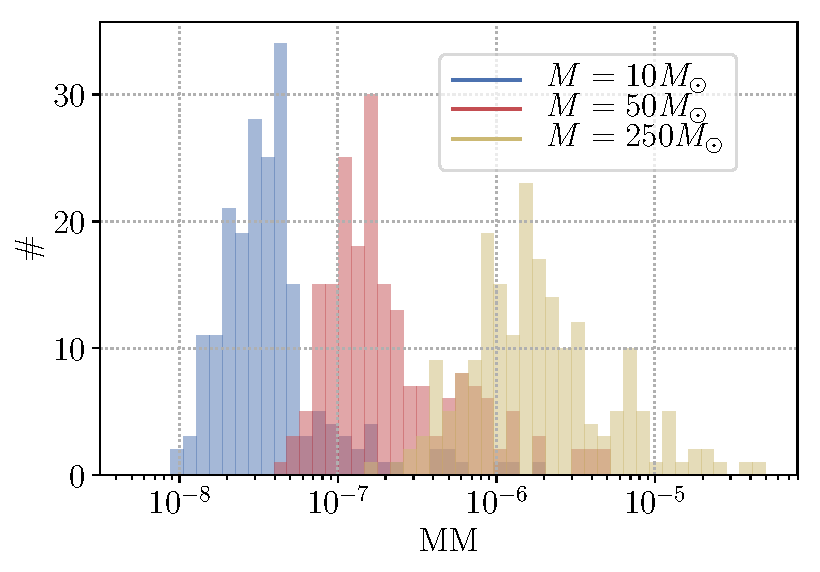
\includegraphics[width=.99\linewidth]{../plots/plot_MM_ROM.pdf}
  \caption{Unfaithfulness of ROM waveforms compared to the original EOBNRv2HM waveforms, computed as in~\eqref{}. We show here the results for the orientations \SM{[complete]}, for 200 random mass ratio values between 1 and 12, for masses $10 \Msol$, $50 \Msol$ and $250 \Msol$. The inclination angle is $\iota = \pi/2$, maximizing the effect of higher harmonics.}
  \label{fig:MMROM}
\end{figure}

%%%%%%%%%%%%%%%%%%%%%%%%%%%%%%%%%%%%
%%%%%%%%%%%%%%%%%%%%%%%%%%%%%%%%%%%%

\section{SNR dependence of parameter estimation}
\label{sec:SMBHPEdistance}

-- show series of analyses varying only the distance/SNR

\begin{figure*}
  \centering
  \begin{minipage}{.32\linewidth}
      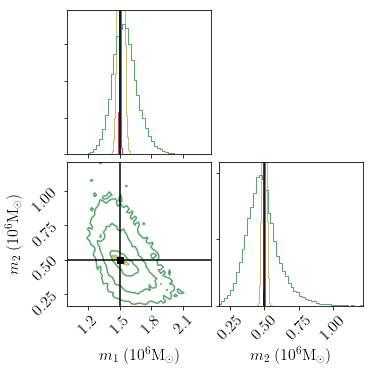
\includegraphics[width=.99\linewidth]{../plots/corner_smbh_case9_hm_dseries_m1m2.png}
   \end{minipage}
   \begin{minipage}{.32\linewidth}
      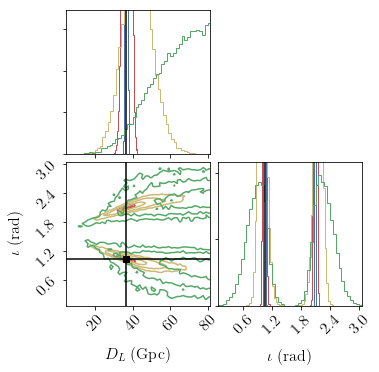
\includegraphics[width=.99\linewidth]{../plots/corner_smbh_case9_hm_dseries_Dinc.png}
   \end{minipage}
   \begin{minipage}{.32\linewidth}
      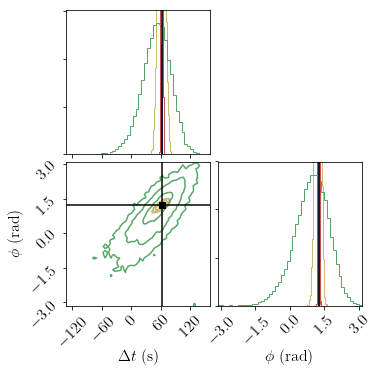
\includegraphics[width=.99\linewidth]{../plots/corner_smbh_case9_hm_dseries_tphi.png}
   \end{minipage}
  \caption{.}
  \label{fig:smbhCornerZoomHMCase9}
\end{figure*}

\begin{figure*}
  \centering
  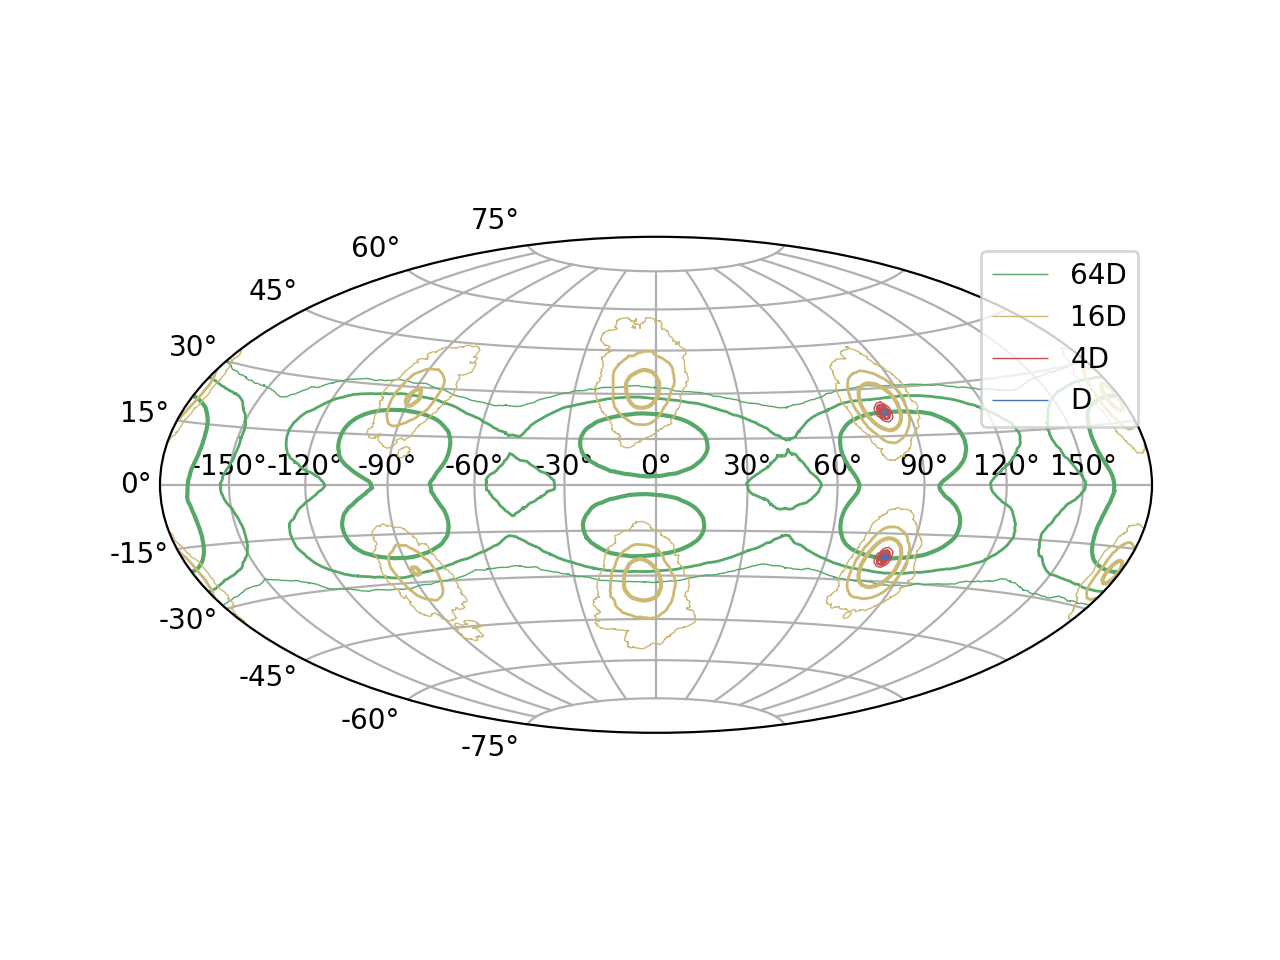
\includegraphics[width=.8\linewidth]{../plots/plot_mollweide_dseries.png}
  \caption{.}
  \label{fig:MollweidesmbhTserieshmCase9}
\end{figure*}

%%%%%%%%%%%%%%%%%%%%%%%%%%%%%%%%%%%%
%%%%%%%%%%%%%%%%%%%%%%%%%%%%%%%%%%%%

\begin{acknowledgments}

TDC was supported by an appointment to the NASA Postdoctoral Program at the
Goddard Space Flight Center, administered by Universities Space Research
Association under contract with NASA.

\end{acknowledgments}

\bibliography{references.bib}

\end{document}
